\chapter{PENGUJIAN DAN ANALISIS}
\label{chap:pengujiananalisis}

% Ubah bagian-bagian berikut dengan isi dari pengujian dan analisis

Pada bab ini, dipaparkan mengenai data hasil pengujian beserta analisis dari setiap pelaksanaan yang dilakukan berdasarkan tahapan yang telah dijelaskan pada bab sebelumnya mengenai metodologi serta dipaparkan juga mengenai beberapa skenario pengujian yang telah diterapkan. Skenario pengujian yang dilakukan berguna untuk mengetahui performa dan tingkat akurasi dari model beserta sistem yang telah dibuat berdasarkan tahapan yang dijelaskan pada metodologi. Skenario pengujian yang diterapkan meliputi beberapa poin sebagai berikut:

\begin{enumerate}[topsep=8pt,itemsep=4pt,partopsep=4pt, parsep=4pt]
  \item Pengujian Performa Model dengan menggunakan \emph{Confusion Matrix}
  \item Pengujian Performa Model dengan menggunakan Variasi Jarak
  \item Pengujian Performa Model dengan menggunakan Variasi Pencahayaan
  \item Pengujian Performa \emph{Frame Per Second} (FPS) pada Sistem Kontrol Kursi Roda
  \item Pengujian Waktu dari \emph{Inference Time} pada Model ke \emph{Response Time} pada Motor Kursi Roda
  \item Pengujian Kestabilan pada Motor Kursi Roda
\end{enumerate}

Penerapan metodologi beserta skenario pengujian yang dijelaskan dan dianalisa pada bab ini diharapkan dapat memberikan pemahaman terkait hasil akhir berupa kesimpulan dan saran yang didapat sehingga penelitian ini dapat dievaluasi dan terus dikembangkan.

\section{Pengujian}
\label{sec:skenariopengujian}

Pada sub-bab ini, dipaparkan mengenai hasil dari skenario pengujian yang telah dilakukan terhadap model, motor kursi roda, beserta keseluruhan sistem kontrol kursi roda. Hasil pengujian yang didapatkan berupa data yang kemudian dapat dianalisa dan diolah sehingga diketahui performa dan tingkat akurasi yang dapat digunakan sebagai dasar untuk pengembangan penelitian lebih lanjut serta menarik kesimpulan dan saran secara keseluruhan. Pengujian yang dilakukan dijelaskan sebagai berikut:

\section{Pengujian Performa Model dengan menggunakan \emph{Confusion Matrix}}

Pada penelitian ini digunakan metode \emph{Convolutional Neural Network} (CNN) untuk membuat model. Selama pembuatan model CNN, dilakukan pengambilan dan pengelompokan data citra yang kemudian digunakan sebagai \emph{dataset} untuk pelatihan dan validasi model CNN. Data yang dilatih berupa citra \emph{landmark} mata yang telah dikelompokkan menjadi lima kelas seperti yang telah dipaparkan pada metodologi. Lima kelas yang mengelompokkan data citra \emph{landmark} mata adalah 'Kanan', 'Kiri', 'Maju', 'Mundur', dan 'Stop'.

\emph{Dataset} yang digunakan dalam penelitian ini terdiri dari data citra yang berjumlah 2000 data, dimana kemudian data citra tersebut dikelompokkan berdasarkan lima kelas sehingga jumlahnya masing-masing 400 data per kelas. Data-data citra tersebut dimasukkan ke dalam lima folder dengan label sesuai dengan nama kelas yang dipaparkan sebelumnya. Selanjutnya dalam masing-masing folder kelas, 400 data citra tersebut dibagi (\emph{split}) dengan bobot 70\% untuk data \emph{training} (pelatihan) sehingga berjumlah 280 data citra yang dimasukkan pada folder \emph{training }dan bobot 30\% untuk data \emph{validation} (validasi) sehingga berjumlah 120 data citra yang dimasukkan dalam folder \emph{validation}. Kelima folder kelas tersebut akan digunakan sebagai \emph{input} data \emph{training} dan data \emph{validation} dalam pembuatan model.

Secara keseluruhan, \emph{dataset} citra \emph{landmark} mata yang digunakan dalam penelitian ini, berjumlah 2000 data citra yang dibagi ke dalam 5 kelas, dengan pembagian data pelatihan sebanyak 280 data citra dan data validasi sebanyak 120 data citra. Visualisasi pembagian \emph{dataset} yang digunakan pada penelitian ini dapat dilihat pada Gambar \ref{fig:dataset} beserta rinciannya pada Tabel \ref{tb:datadiagram}.

%Gambar 4.1
\begin{figure} [ht] \centering
  % Nama dari file gambar yang diinputkan
  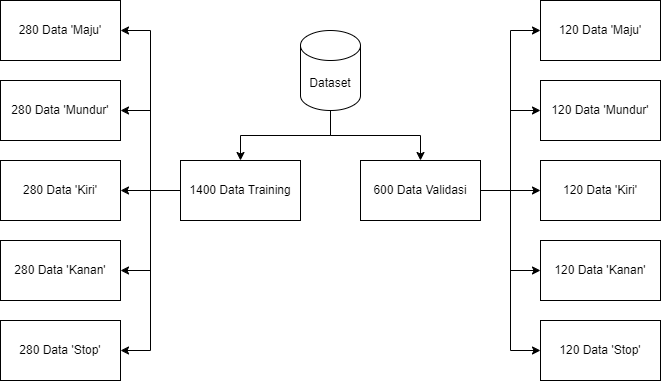
\includegraphics[width=1\textwidth]{gambar/bab4/visualdataset.png}
  % Keterangan gambar yang diinputkan
  \caption{Diagram Pembagian \emph{Dataset}}
  % Label referensi dari gambar yang diinputkan
  \label{fig:dataset}
\end{figure}

%Tabel 4.1
\begin{longtable}{|c|c|c|}
  \caption{\emph{Dataset} Kontrol {Kursi Roda}}
  \label{tb:datadiagram} \\
  \hline
  \rowcolor[HTML]{C0C0C0}
  \textbf{Kelas Kontrol} & \textbf{Data Pelatihan} & \textbf{Data Validasi} \\ \hline
  Kanan            & 280 Citra               & 120 Citra               \\ \hline
  Kiri              & 280 Citra               & 120 Citra               \\ \hline
  Maju             & 280 Citra               & 120 Citra               \\ \hline
  Mundur            & 280 Citra               & 120 Citra               \\ \hline
  Stop             & 280 Citra               & 120 Citra               \\ \hline
\end{longtable}

Selanjutnya, setelah proses akuisisi data telah dilakukan, model CNN dibangun dengan menggunakan \emph{dataset} pelatihan dan \emph{dataset} validasi yang sebelumnya telah diambil sebagai data pelatihan dan data pengujian. Dalam pembuatan model CNN, proses pelatihan dilakukan dengan menggunakan model CNN yang terdiri dari sebelas lapisan seperti struktur yang telah dipaparkan pada metodologi penelitian. Pelatihan pada model CNN dilakukan dengan konfigurasi 40 tahapan \emph{epoch} dengan 10 langkah pelatihan per \emph{epoch}. Ditambahkan juga modul \emph{early stopping} selama pelatihan model agar didapatkan model terbaik, yaitu pada \emph{epoch} ke-30. Berdasarkan hasil pelatihan tersebut, dihasilkan nilai akurasi sebesar 100\% dengan akurasi pengujian sebesar 99.83\%. Selain itu, hasil pelatihan juga menunjukkan nilai \emph{loss} sebesar 0.22\% dengan \emph{loss} pengujian sebesar 1.14\%. Variabel tersebut dapat dilihat pada Gambar \ref{fig:acc_loss} yang telah memvisualisasikan hasil akurasi dan akurasi pengujian serta hasil \emph{loss} dan \emph{loss} pengujian dalam bentuk grafik dengan nilai akurasi, akurasi pengujian, \emph{loss}, dan \emph{loss} pengujian terhadap tiap tahapan \emph{epoch}.

%Gambar 4.2
\begin{figure}[ht]
  \centering
  \begin{subfigure}[b]{0.72\textwidth}
      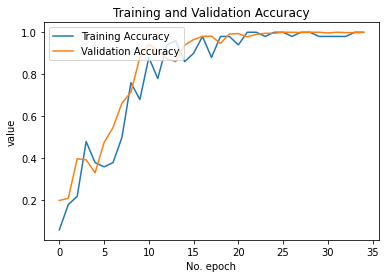
\includegraphics[width=\textwidth]{gambar/bab4/model5 (30cm)/train.png}
      \caption{Akurasi}
  \end{subfigure}

  \begin{subfigure}[b]{0.72\textwidth}
      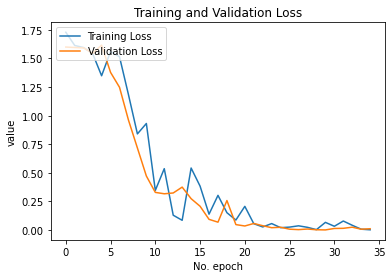
\includegraphics[width=\textwidth]{gambar/bab4/model5 (30cm)/loss.png}
      \caption{\emph{Loss}}
  \end{subfigure}
  \caption{Grafik Akurasi dan \emph{Loss} pada Hasil Pelatihan Model}
  \label{fig:acc_loss}
\end{figure}

Setelah didapatkan grafik akurasi dan \emph{loss} untuk hasil pelatihan model, selanjutnya dilakukan perhitungan untuk \emph{confusion matrix} yang dibuat berdasarkan \emph{dataset} validasi. \emph{Confusion matrix} dihitung dengan membandingkan label yang sebenarnya (\emph{true label}) dengan label yang diprediksi (\emph{predicted label}) yang kemudian kedua label tersebut akan divisualisasikan menjadi \emph{matrix} yang dibagi menjadi tiap kelas kontrol, dimana \emph{predicted label} menjadi sumbu X dan \emph{true label} menjadi sumbu Y. Dari visualisasi \emph{confusion matrix}, dapat diamati bahwa keseluruhan 600 \emph{dataset} validasi yang telah diuji berdasarkan label yang sebenarnya sudah terprediksi dengan benar.

%Gambar 4.3
\begin{figure} [ht] \centering
  % Nama dari file gambar yang diinputkan
  \includegraphics[width=0.45\textwidth]{gambar/bab4/model5 (30cm)/matrix.png}
  % Keterangan gambar yang diinputkan
  \caption{\emph{Confusion Matrix} Model Hasil Pelatihan}
  % Label referensi dari gambar yang diinputkan
  \label{fig:matrix1}
\end{figure}

Kemudian dari \emph{confusion matrix}, didapatkan hasil klasifikasi yang dapat dikelompokkan menjadi beberapa parameter yaitu \emph{true positive}, \emph{true negative}, \emph{false positive}, dan \emph{false negative}. \emph{True positive} adalah hasil dimana model memprediksi kelas positif dengan benar. Demikian pula, \emph{true negative} adalah hasil dimana model memprediksi kelas negatif dengan benar. Kelas positif adalah kelas itu sendiri, sedangkan kelas negatif adalah kelas lain selain kelas itu sendiri. \emph{False positive} adalah hasil di mana model salah memprediksi kelas positif. Dan \emph{false negative} adalah hasil di mana model salah memprediksi kelas negatif. Hasil klasifikasi dapat dilihat pada Tabel \ref{tb:cm_model} di bawah.

%Tabel 4.2
\begin{longtable}{|l|c|c|c|c|}
  \caption{Hasil klasifikasi model dengan \emph{confusion matrix}}
  \label{tb:cm_model} \\
  \hline
  \rowcolor[HTML]{C0C0C0} 
  \textbf{Kelas} & \textbf{TP} & \textbf{TN} & \textbf{FP} & \textbf{FN} \\ \hline
  Kanan    & 120          & 480         & 0           & 0           \\ \hline
  Kiri      & 120          & 480         & 0           & 0           \\ \hline
  Maju      & 120          & 480         & 0           & 0           \\ \hline
  Mundur     & 120          & 480         & 0           & 0           \\ \hline
  Stop  & 120          & 480         & 0           & 0           \\ \hline
\end{longtable}

Berdasarkan Tabel \ref{tb:cm_model} diatas, dapat dilihat pada semua kelas memiliki 120 data citra yang termasuk dalam \emph{true positive}, 480 data citra yang termasuk dalam \emph{true negative}, 0 data citra yang termasuk dalam \emph{false positive}, dan 0 data citra yang termasuk dalam \emph{false negative}. 

Dari hasil klasifikasi tersebut, selanjutnya dapat dihitung nilai validasi model. Nilai validasi yang dihitung yaitu \emph{accuracy}, \emph{precision}, \emph{recall}, dan \emph{f-1 score}. Penggambaran lebih detail dapat dilihat pada Tabel \ref{tb:vs_model}

%Tabel 4.3
\begin{longtable}{|l|c|c|c|c|}
  \caption{Hasil validasi nilai model}
  \label{tb:vs_model} \\
  \hline
  \rowcolor[HTML]{C0C0C0} 
  \textbf{Kelas} & \textbf{Accuracy} & \textbf{Precision} & \textbf{Recall} & \textbf{F1-Score} \\ \hline
  Kanan    & 100\%            & 100\%             & 100\%           & 100\%            \\ \hline
  Kiri     & 100\%          & 100\%           & 100\%           & 100\%           \\ \hline
  Maju      & 100\%          & 100\%           & 100\%          & 100\%          \\ \hline
  Mundur     & 100\%            & 100\%             & 100\%           & 100\%            \\ \hline
  Stop  & 100\%            & 100\%             & 100\%           & 100\%            \\ \hline
\end{longtable}

Dilihat dari Tabel \ref{tb:vs_model}, nilai \emph{accuracy}, \emph{precision}, \emph{recall}, dan \emph{f1-score} pada semua kelas bernilai sama. Untuk kelas 'Kanan' , didapatkan nilai \emph{accuracy} sebesar 100\%, nilai \emph{precision} sebesar 100\%, nilai \emph{recall} sebesar 100\%, dan nilai \emph{f1-score} sebesar 100\%. Kemudian untuk kelas 'Kiri' , didapatkan nilai \emph{accuracy} sebesar 100\%, nilai \emph{precision} sebesar 100\%, nilai \emph{recall} sebesar 100\%, dan nilai \emph{f1-score} sebesar 100\%. Selanjutnya pada kelas 'Maju' , didapatkan nilai \emph{accuracy} sebesar 100\%, nilai \emph{precision} sebesar 100\%, nilai \emph{recall} sebesar 100\%, dan nilai \emph{f1-score} sebesar 100\%. Untuk kelas 'Mundur' , didapatkan nilai \emph{accuracy} sebesar 100\%, nilai \emph{precision} sebesar 100\%, nilai \emph{recall} sebesar 100\%, dan nilai \emph{f1-score} sebesar 100\%. Terakhir pada kelas 'Stop' , didapatkan nilai \emph{accuracy} sebesar 100\%, nilai \emph{precision} sebesar 100\%, nilai \emph{recall} sebesar 100\%, dan nilai \emph{f1-score} sebesar 100\%. Nilai validasi tersebut bisa didapatkan karena nilai \emph{true positive}, \emph{true negative}, \emph{false positive}, dan \emph{false negative} dari \emph{confusion matrix} yang dipaparkan pada Tabel \ref{tb:cm_model} memiliki nilai prediksi yang baik untuk kelima kelas.


\section{Pengujian Performa Model dengan menggunakan Variasi Jarak}

Pada skenario pengujian selanjutnya, model diuji berdasarkan beberapa variasi jarak. Pengujian jarak berguna untuk mengetahui performa dan tingkat akurasi model jika diuji berdasarkan input citra dari jarak yang berbeda-beda. Hal ini perlu diuji karena semakin jauh jarak pendeteksi citra, maka semakin kecil data visual citra yang diperoleh.

\subsection{Jarak 30 cm}

%Gambar 4.4
\begin{figure} [ht] \centering
  % Nama dari file gambar yang diinputkan
  \includegraphics[width=0.25\textwidth]{gambar/bab4/model5 (30cm)/matrix.png}
  % Keterangan gambar yang diinputkan
  \caption{\emph{Confusion Matrix} Model Hasil Pelatihan}
  % Label referensi dari gambar yang diinputkan
  \label{fig:matrix2}
\end{figure}

%Tabel 4.4
\begin{longtable}{|l|c|c|c|c|}
  \caption{Hasil klasifikasi model dengan \emph{confusion matrix}}
  \label{tb:cm_model2} \\
  \hline
  \rowcolor[HTML]{C0C0C0} 
  \textbf{Kelas} & \textbf{TP} & \textbf{TN} & \textbf{FP} & \textbf{FN} \\ \hline
  Kanan    & 120          & 480         & 0           & 0           \\ \hline
  Kiri      & 120          & 480         & 0           & 0           \\ \hline
  Maju      & 120          & 480         & 0           & 0           \\ \hline
  Mundur     & 120          & 480         & 0           & 0           \\ \hline
  Stop  & 120          & 480         & 0           & 0           \\ \hline
\end{longtable}

%Tabel 4.5
\begin{longtable}{|l|c|c|c|c|}
  \caption{Hasil validasi nilai model}
  \label{tb:vs_model2} \\
  \hline
  \rowcolor[HTML]{C0C0C0} 
  \textbf{Kelas} & \textbf{Accuracy} & \textbf{Precision} & \textbf{Recall} & \textbf{F1-Score} \\ \hline
  Kanan    & 100\%            & 100\%             & 100\%           & 100\%            \\ \hline
  Kiri     & 100\%          & 100\%           & 100\%           & 100\%           \\ \hline
  Maju      & 100\%          & 100\%           & 100\%          & 100\%          \\ \hline
  Mundur     & 100\%            & 100\%             & 100\%           & 100\%            \\ \hline
  Stop  & 100\%            & 100\%             & 100\%           & 100\%            \\ \hline
\end{longtable}

\subsection{Jarak 50 cm}

%Gambar 4.5
\begin{figure} [ht] \centering
  % Nama dari file gambar yang diinputkan
  \includegraphics[width=0.25\textwidth]{gambar/bab4/model6 (50cm)/matrix.png}
  % Keterangan gambar yang diinputkan
  \caption{\emph{Confusion Matrix} Model Hasil Pelatihan}
  % Label referensi dari gambar yang diinputkan
  \label{fig:matrix3}
\end{figure}

%Tabel 4.6
\begin{longtable}{|l|c|c|c|c|}
  \caption{Hasil klasifikasi model dengan \emph{confusion matrix}}
  \label{tb:cm_model3} \\
  \hline
  \rowcolor[HTML]{C0C0C0} 
  \textbf{Kelas} & \textbf{TP} & \textbf{TN} & \textbf{FP} & \textbf{FN} \\ \hline
  Kanan    & 120          & 480         & 0           & 0           \\ \hline
  Kiri      & 120          & 480         & 0           & 0           \\ \hline
  Maju      & 120          & 480         & 0           & 0           \\ \hline
  Mundur     & 120          & 480         & 0           & 0           \\ \hline
  Stop  & 120          & 480         & 0           & 0           \\ \hline
\end{longtable}

%Tabel 4.7
\begin{longtable}{|l|c|c|c|c|}
  \caption{Hasil validasi nilai model}
  \label{tb:vs_model3} \\
  \hline
  \rowcolor[HTML]{C0C0C0} 
  \textbf{Kelas} & \textbf{Accuracy} & \textbf{Precision} & \textbf{Recall} & \textbf{F1-Score} \\ \hline
  Kanan    & 100\%            & 100\%             & 100\%           & 100\%            \\ \hline
  Kiri     & 100\%          & 100\%           & 100\%           & 100\%           \\ \hline
  Maju      & 100\%          & 100\%           & 100\%          & 100\%          \\ \hline
  Mundur     & 100\%            & 100\%             & 100\%           & 100\%            \\ \hline
  Stop  & 100\%            & 100\%             & 100\%           & 100\%            \\ \hline
\end{longtable}

\subsection{Jarak 70 cm}

%Gambar 4.6
\begin{figure} [ht] \centering
  % Nama dari file gambar yang diinputkan
  \includegraphics[width=0.25\textwidth]{gambar/bab4/model7 (70cm)/matrix.png}
  % Keterangan gambar yang diinputkan
  \caption{\emph{Confusion Matrix} Model Hasil Pelatihan}
  % Label referensi dari gambar yang diinputkan
  \label{fig:matrix4}
\end{figure}

%Tabel 4.8
\begin{longtable}{|l|c|c|c|c|}
  \caption{Hasil klasifikasi model dengan \emph{confusion matrix}}
  \label{tb:cm_model4} \\
  \hline
  \rowcolor[HTML]{C0C0C0} 
  \textbf{Kelas} & \textbf{TP} & \textbf{TN} & \textbf{FP} & \textbf{FN} \\ \hline
  Kanan    & 120          & 480         & 0           & 0           \\ \hline
  Kiri      & 120          & 480         & 0           & 0           \\ \hline
  Maju      & 120          & 480         & 0           & 0           \\ \hline
  Mundur     & 120          & 480         & 0           & 0           \\ \hline
  Stop  & 120          & 480         & 0           & 0           \\ \hline
\end{longtable}

%Tabel 4.9
\begin{longtable}{|l|c|c|c|c|}
  \caption{Hasil validasi nilai model}
  \label{tb:vs_model4} \\
  \hline
  \rowcolor[HTML]{C0C0C0} 
  \textbf{Kelas} & \textbf{Accuracy} & \textbf{Precision} & \textbf{Recall} & \textbf{F1-Score} \\ \hline
  Kanan    & 100\%            & 100\%             & 100\%           & 100\%            \\ \hline
  Kiri     & 100\%          & 100\%           & 100\%           & 100\%           \\ \hline
  Maju      & 100\%          & 100\%           & 100\%          & 100\%          \\ \hline
  Mundur     & 100\%            & 100\%             & 100\%           & 100\%            \\ \hline
  Stop  & 100\%            & 100\%             & 100\%           & 100\%            \\ \hline
\end{longtable}

\subsection{Jarak 90 cm}

%Gambar 4.7
\begin{figure} [ht] \centering
  % Nama dari file gambar yang diinputkan
  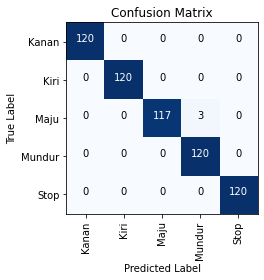
\includegraphics[width=0.25\textwidth]{gambar/bab4/model8 (90cm)/matrix.png}
  % Keterangan gambar yang diinputkan
  \caption{\emph{Confusion Matrix} Model Hasil Pelatihan}
  % Label referensi dari gambar yang diinputkan
  \label{fig:matrix5}
\end{figure}

%Tabel 4.10
\begin{longtable}{|l|c|c|c|c|}
  \caption{Hasil klasifikasi model dengan \emph{confusion matrix}}
  \label{tb:cm_model5} \\
  \hline
  \rowcolor[HTML]{C0C0C0} 
  \textbf{Kelas} & \textbf{TP} & \textbf{TN} & \textbf{FP} & \textbf{FN} \\ \hline
  Kanan    & 120          & 480         & 0           & 0           \\ \hline
  Kiri      & 120          & 480         & 0           & 0           \\ \hline
  Maju      & 117          & 480         & 0           & 3           \\ \hline
  Mundur     & 120          & 477         & 3           & 0           \\ \hline
  Stop  & 120          & 480         & 0           & 0           \\ \hline
\end{longtable}

%Tabel 4.11
\begin{longtable}{|l|c|c|c|c|}
  \caption{Hasil validasi nilai model}
  \label{tb:vs_model5} \\
  \hline
  \rowcolor[HTML]{C0C0C0} 
  \textbf{Kelas} & \textbf{Accuracy} & \textbf{Precision} & \textbf{Recall} & \textbf{F1-Score} \\ \hline
  Kanan    & 100\%            & 100\%             & 100\%           & 100\%            \\ \hline
  Kiri     & 100\%          & 100\%           & 100\%           & 100\%           \\ \hline
  Maju      & 99.50\%          & 100\%           & 97.50\%          & 98.73\%          \\ \hline
  Mundur     & 99.50\%            & 97.56\%             & 100\%           & 98.77\%            \\ \hline
  Stop  & 100\%            & 100\%             & 100\%           & 100\%            \\ \hline
\end{longtable}

\subsection{Jarak 110 cm}

%Gambar 4.8
\begin{figure} [ht] \centering
  % Nama dari file gambar yang diinputkan
  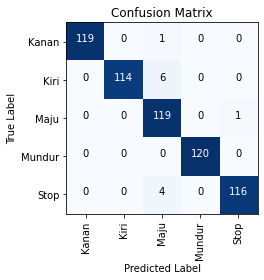
\includegraphics[width=0.25\textwidth]{gambar/bab4/model5 (30cm)/110cm/matrix.png}
  % Keterangan gambar yang diinputkan
  \caption{\emph{Confusion Matrix} Model Hasil Pelatihan}
  % Label referensi dari gambar yang diinputkan
  \label{fig:matrix6}
\end{figure}

%Tabel 4.12
\begin{longtable}{|l|c|c|c|c|}
  \caption{Hasil klasifikasi model dengan \emph{confusion matrix}}
  \label{tb:cm_model6} \\
  \hline
  \rowcolor[HTML]{C0C0C0} 
  \textbf{Kelas} & \textbf{TP} & \textbf{TN} & \textbf{FP} & \textbf{FN} \\ \hline
  Kanan    & 119          & 480         & 0           & 1           \\ \hline
  Kiri      & 114          & 480         & 0           & 6           \\ \hline
  Maju      & 119          & 469         & 11           & 1           \\ \hline
  Mundur     & 120          & 480         & 0           & 0           \\ \hline
  Stop  & 116          & 479         & 1           & 4           \\ \hline
\end{longtable}

%Tabel 4.13
\begin{longtable}{|l|c|c|c|c|}
  \caption{Hasil validasi nilai model}
  \label{tb:vs_model6} \\
  \hline
  \rowcolor[HTML]{C0C0C0} 
  \textbf{Kelas} & \textbf{Accuracy} & \textbf{Precision} & \textbf{Recall} & \textbf{F1-Score} \\ \hline
  Kanan    & 99.83\%            & 100\%             & 99.17\%           & 99.58\%            \\ \hline
  Kiri     & 99\%          & 100\%           & 95\%           & 97.44\%           \\ \hline
  Maju      & 98\%          & 91.54\%           & 99.17\%          & 95.20\%          \\ \hline
  Mundur     & 100\%            & 100\%             & 100\%           & 100\%            \\ \hline
  Stop  & 99.17\%            & 99.15\%             & 96.67\%           & 97.89\%            \\ \hline
\end{longtable}

\section{Pengujian Performa Model dengan menggunakan Variasi Pencahayaan}

%Tabel 4.14
\subsection{Pengujian pada cahaya 35 Lux}
\begin{longtable}{|l|c|}
  \caption{Hasil pengujian kelas kanan pada 35 Lux}
  \label{tb:luxkanan} \\
  \hline
  \rowcolor[HTML]{C0C0C0} 
  \textbf{Kelas} & \textbf{Detection State}                           \\ \hline
  Kanan          & Frame detected!: Class ID = 0, Class Name = Kanan \\ \hline
  Kanan          & Frame detected!: Class ID = 0, Class Name = Kanan \\ \hline
  Kanan          & Frame detected!: Class ID = 0, Class Name = Kanan \\ \hline
  Kanan          & Frame detected!: Class ID = 0, Class Name = Kanan \\ \hline
  Kanan          & Frame detected!: Class ID = 0, Class Name = Kanan \\ \hline
  Kanan          & Frame detected!: Class ID = 0, Class Name = Kanan \\ \hline
  Kanan          & Frame detected!: Class ID = 0, Class Name = Kanan \\ \hline
  Kanan          & Frame detected!: Class ID = 0, Class Name = Kanan \\ \hline
  Kanan          & Frame detected!: Class ID = 0, Class Name = Kanan \\ \hline
  Kanan          & Frame detected!: Class ID = 0, Class Name = Kanan \\ \hline
  Kanan          & Frame detected!: Class ID = 0, Class Name = Kanan \\ \hline
  Kanan          & Frame detected!: Class ID = 0, Class Name = Kanan \\ \hline
  Kanan          & Frame detected!: Class ID = 0, Class Name = Kanan \\ \hline
  Kanan          & Frame detected!: Class ID = 0, Class Name = Kanan \\ \hline
  Kanan          & Frame detected!: Class ID = 0, Class Name = Kanan \\ \hline
  Kanan          & Frame detected!: Class ID = 0, Class Name = Kanan \\ \hline
  Kanan          & Frame detected!: Class ID = 0, Class Name = Kanan \\ \hline
  Kanan          & Frame detected!: Class ID = 0, Class Name = Kanan \\ \hline
  Kanan          & Frame detected!: Class ID = 0, Class Name = Kanan \\ \hline
  Kanan          & Frame detected!: Class ID = 0, Class Name = Kanan \\ \hline
  Kanan          & Frame detected!: Class ID = 0, Class Name = Kanan \\ \hline
  Kanan          & Frame detected!: Class ID = 0, Class Name = Kanan \\ \hline
  Kanan          & Frame detected!: Class ID = 0, Class Name = Kanan \\ \hline
  Kanan          & Frame detected!: Class ID = 0, Class Name = Kanan \\ \hline
  Kanan          & Frame detected!: Class ID = 0, Class Name = Kanan \\ \hline
  Kanan          & Frame detected!: Class ID = 0, Class Name = Kanan \\ \hline
  Kanan          & Frame detected!: Class ID = 0, Class Name = Kanan \\ \hline
  Kanan          & Frame detected!: Class ID = 0, Class Name = Kanan \\ \hline
  Kanan          & Frame detected!: Class ID = 0, Class Name = Kanan \\ \hline
  Kanan          & Frame detected!: Class ID = 0, Class Name = Kanan \\ \hline
\end{longtable}

%Tabel 4.15
\begin{longtable}{|l|c|}
  \caption{Hasil pengujian kelas kiri pada 35 Lux}
  \label{tb:luxkiri} \\
  \hline
  \rowcolor[HTML]{C0C0C0} 
  \textbf{Kelas} & \textbf{Detection State}                           \\ \hline
  Kiri           & Frame detected!: Class ID = 1, Class Name = Kiri \\ \hline
  Kiri           & Frame detected!: Class ID = 1, Class Name = Kiri \\ \hline
  Kiri           & Frame detected!: Class ID = 1, Class Name = Kiri \\ \hline
  Kiri           & Frame detected!: Class ID = 1, Class Name = Kiri \\ \hline
  Kiri           & Frame detected!: Class ID = 1, Class Name = Kiri \\ \hline
  Kiri           & Frame detected!: Class ID = 1, Class Name = Kiri \\ \hline
  Kiri           & Frame detected!: Class ID = 1, Class Name = Kiri \\ \hline
  Kiri           & Frame detected!: Class ID = 1, Class Name = Kiri \\ \hline
  Kiri           & Frame detected!: Class ID = 1, Class Name = Kiri \\ \hline
  Kiri           & Frame detected!: Class ID = 1, Class Name = Kiri \\ \hline
  Kiri           & Frame detected!: Class ID = 1, Class Name = Kiri \\ \hline
  Kiri           & Frame detected!: Class ID = 1, Class Name = Kiri \\ \hline
  Kiri           & Frame detected!: Class ID = 1, Class Name = Kiri \\ \hline
  Kiri           & Frame detected!: Class ID = 1, Class Name = Kiri \\ \hline
  Kiri           & Frame detected!: Class ID = 1, Class Name = Kiri \\ \hline
  Kiri           & Frame detected!: Class ID = 1, Class Name = Kiri \\ \hline
  Kiri           & Frame detected!: Class ID = 1, Class Name = Kiri \\ \hline
  Kiri           & Frame detected!: Class ID = 1, Class Name = Kiri \\ \hline
  Kiri           & Frame detected!: Class ID = 1, Class Name = Kiri \\ \hline
  Kiri           & Frame detected!: Class ID = 1, Class Name = Kiri \\ \hline
  Kiri           & Frame detected!: Class ID = 1, Class Name = Kiri \\ \hline
  Kiri           & Frame detected!: Class ID = 1, Class Name = Kiri \\ \hline
  Kiri           & Frame detected!: Class ID = 1, Class Name = Kiri \\ \hline
  Kiri           & Frame detected!: Class ID = 1, Class Name = Kiri \\ \hline
  Kiri           & Frame detected!: Class ID = 1, Class Name = Kiri \\ \hline
  Kiri           & Frame detected!: Class ID = 1, Class Name = Kiri \\ \hline
  Kiri           & Frame detected!: Class ID = 1, Class Name = Kiri \\ \hline
  Kiri           & Frame detected!: Class ID = 1, Class Name = Kiri \\ \hline
  Kiri           & Frame detected!: Class ID = 1, Class Name = Kiri \\ \hline
  Kiri           & Frame detected!: Class ID = 1, Class Name = Kiri \\ \hline
\end{longtable}

%Tabel 4.16
\begin{longtable}{|l|c|}
  \caption{Hasil pengujian kelas maju pada 35 Lux}
  \label{tb:luxmaju} \\
  \hline
  \rowcolor[HTML]{C0C0C0} 
  \textbf{Kelas} & \textbf{Detection State}                           \\ \hline
  Maju           & Frame detected!: Class ID = 2, Class Name = Maju   \\ \hline
  Maju           & Frame detected!: Class ID = 2, Class Name = Maju   \\ \hline
  Maju           & Frame detected!: Class ID = 2, Class Name = Maju   \\ \hline
  Maju           & Frame detected!: Class ID = 2, Class Name = Maju   \\ \hline
  Maju           & Frame detected!: Class ID = 2, Class Name = Maju   \\ \hline
  Maju           & Frame detected!: Class ID = 2, Class Name = Maju   \\ \hline
  Maju           & Frame detected!: Class ID = 2, Class Name = Maju   \\ \hline
  Maju           & Frame detected!: Class ID = 2, Class Name = Maju   \\ \hline
  Maju           & Frame detected!: Class ID = 3, Class Name = Mundur \\ \hline
  Maju           & Frame detected!: Class ID = 2, Class Name = Maju   \\ \hline
  Maju           & Frame detected!: Class ID = 2, Class Name = Maju   \\ \hline
  Maju           & Frame detected!: Class ID = 2, Class Name = Maju   \\ \hline
  Maju           & Frame detected!: Class ID = 2, Class Name = Maju   \\ \hline
  Maju           & Frame detected!: Class ID = 2, Class Name = Maju   \\ \hline
  Maju           & Frame detected!: Class ID = 2, Class Name = Maju   \\ \hline
  Maju           & Frame detected!: Class ID = 2, Class Name = Maju   \\ \hline
  Maju           & Frame detected!: Class ID = 3, Class Name = Mundur \\ \hline
  Maju           & Frame detected!: Class ID = 2, Class Name = Maju   \\ \hline
  Maju           & Frame detected!: Class ID = 2, Class Name = Maju   \\ \hline
  Maju           & Frame detected!: Class ID = 2, Class Name = Maju   \\ \hline
  Maju           & Frame detected!: Class ID = 2, Class Name = Maju   \\ \hline
  Maju           & Frame detected!: Class ID = 2, Class Name = Maju   \\ \hline
  Maju           & Frame detected!: Class ID = 3, Class Name = Mundur \\ \hline
  Maju           & Frame detected!: Class ID = 2, Class Name = Maju   \\ \hline
  Maju           & Frame detected!: Class ID = 2, Class Name = Maju   \\ \hline
  Maju           & Frame detected!: Class ID = 2, Class Name = Maju   \\ \hline
  Maju           & Frame detected!: Class ID = 2, Class Name = Maju   \\ \hline
  Maju           & Frame detected!: Class ID = 2, Class Name = Maju   \\ \hline
  Maju           & Frame detected!: Class ID = 2, Class Name = Maju   \\ \hline
  Maju           & Frame detected!: Class ID = 2, Class Name = Maju   \\ \hline
\end{longtable}

%Tabel 4.17
\begin{longtable}{|l|c|}
  \caption{Hasil pengujian kelas mundur pada 35 Lux}
  \label{tb:luxmundur} \\
  \hline
  \rowcolor[HTML]{C0C0C0} 
  \textbf{Kelas} & \textbf{Detection State}                           \\ \hline
  Mundur         & Frame detected!: Class ID = 3, Class Name = Mundur \\ \hline
  Mundur         & Frame detected!: Class ID = 3, Class Name = Mundur \\ \hline
  Mundur         & Frame detected!: Class ID = 3, Class Name = Mundur \\ \hline
  Mundur         & Frame detected!: Class ID = 3, Class Name = Mundur \\ \hline
  Mundur         & Frame detected!: Class ID = 3, Class Name = Mundur \\ \hline
  Mundur         & Frame detected!: Class ID = 3, Class Name = Mundur \\ \hline
  Mundur         & Frame detected!: Class ID = 2, Class Name = Maju   \\ \hline
  Mundur         & Frame detected!: Class ID = 3, Class Name = Mundur \\ \hline
  Mundur         & Frame detected!: Class ID = 3, Class Name = Mundur \\ \hline
  Mundur         & Frame detected!: Class ID = 3, Class Name = Mundur \\ \hline
  Mundur         & Frame detected!: Class ID = 3, Class Name = Mundur \\ \hline
  Mundur         & Frame detected!: Class ID = 3, Class Name = Mundur \\ \hline
  Mundur         & Frame detected!: Class ID = 3, Class Name = Mundur \\ \hline
  Mundur         & Frame detected!: Class ID = 3, Class Name = Mundur \\ \hline
  Mundur         & Frame detected!: Class ID = 3, Class Name = Mundur \\ \hline
  Mundur         & Frame detected!: Class ID = 3, Class Name = Mundur \\ \hline
  Mundur         & Frame detected!: Class ID = 3, Class Name = Mundur \\ \hline
  Mundur         & Frame detected!: Class ID = 2, Class Name = Maju   \\ \hline
  Mundur         & Frame detected!: Class ID = 3, Class Name = Mundur \\ \hline
  Mundur         & Frame detected!: Class ID = 3, Class Name = Mundur \\ \hline
  Mundur         & Frame detected!: Class ID = 3, Class Name = Mundur \\ \hline
  Mundur         & Frame detected!: Class ID = 3, Class Name = Mundur \\ \hline
  Mundur         & Frame detected!: Class ID = 3, Class Name = Mundur \\ \hline
  Mundur         & Frame detected!: Class ID = 3, Class Name = Mundur \\ \hline
  Mundur         & Frame detected!: Class ID = 3, Class Name = Mundur \\ \hline
  Mundur         & Frame detected!: Class ID = 3, Class Name = Mundur \\ \hline
  Mundur         & Frame detected!: Class ID = 3, Class Name = Mundur \\ \hline
  Mundur         & Frame detected!: Class ID = 3, Class Name = Mundur \\ \hline
  Mundur         & Frame detected!: Class ID = 3, Class Name = Mundur \\ \hline
  Mundur         & Frame detected!: Class ID = 3, Class Name = Mundur \\ \hline
\end{longtable}

%Tabel 4.18
\begin{longtable}{|l|c|}
  \caption{Hasil pengujian kelas stop pada 35 Lux}
  \label{tb:luxstop} \\
  \hline
  \rowcolor[HTML]{C0C0C0} 
  \textbf{Kelas} & \textbf{Detection State}                           \\ \hline
  Stop           & Frame detected!: Class ID = 4, Class Name = Stop \\ \hline
  Stop           & Frame detected!: Class ID = 4, Class Name = Stop \\ \hline
  Stop           & Frame detected!: Class ID = 4, Class Name = Stop \\ \hline
  Stop           & Frame detected!: Class ID = 4, Class Name = Stop \\ \hline
  Stop           & Frame detected!: Class ID = 4, Class Name = Stop \\ \hline
  Stop           & Frame detected!: Class ID = 4, Class Name = Stop \\ \hline
  Stop           & Frame detected!: Class ID = 4, Class Name = Stop \\ \hline
  Stop           & Frame detected!: Class ID = 4, Class Name = Stop \\ \hline
  Stop           & Frame detected!: Class ID = 4, Class Name = Stop \\ \hline
  Stop           & Frame detected!: Class ID = 4, Class Name = Stop \\ \hline
  Stop           & Frame detected!: Class ID = 4, Class Name = Stop \\ \hline
  Stop           & Frame detected!: Class ID = 4, Class Name = Stop \\ \hline
  Stop           & Frame detected!: Class ID = 4, Class Name = Stop \\ \hline
  Stop           & Frame detected!: Class ID = 4, Class Name = Stop \\ \hline
  Stop           & Frame detected!: Class ID = 4, Class Name = Stop \\ \hline
  Stop           & Frame detected!: Class ID = 4, Class Name = Stop \\ \hline
  Stop           & Frame detected!: Class ID = 4, Class Name = Stop \\ \hline
  Stop           & Frame detected!: Class ID = 4, Class Name = Stop \\ \hline
  Stop           & Frame detected!: Class ID = 4, Class Name = Stop \\ \hline
  Stop           & Frame detected!: Class ID = 4, Class Name = Stop \\ \hline
  Stop           & Frame detected!: Class ID = 4, Class Name = Stop \\ \hline
  Stop           & Frame detected!: Class ID = 4, Class Name = Stop \\ \hline
  Stop           & Frame detected!: Class ID = 4, Class Name = Stop \\ \hline
  Stop           & Frame detected!: Class ID = 4, Class Name = Stop \\ \hline
  Stop           & Frame detected!: Class ID = 4, Class Name = Stop \\ \hline
  Stop           & Frame detected!: Class ID = 4, Class Name = Stop \\ \hline
  Stop           & Frame detected!: Class ID = 4, Class Name = Stop \\ \hline
  Stop           & Frame detected!: Class ID = 4, Class Name = Stop \\ \hline
  Stop           & Frame detected!: Class ID = 4, Class Name = Stop \\ \hline
  Stop           & Frame detected!: Class ID = 4, Class Name = Stop \\ \hline
\end{longtable}

\subsection{Pengujian pada cahaya 77 Lux}

\begin{longtable}{|l|c|}
  \caption{Hasil pengujian kelas kanan pada 77 Lux}
  \label{tb:lux77kanan} \\
  \hline
  \rowcolor[HTML]{C0C0C0} 
  \textbf{Kelas} & \textbf{Detection State}                           \\ \hline
  Kanan          & Frame detected!: Class ID = 0, Class Name = Kanan \\ \hline
  Kanan          & Frame detected!: Class ID = 0, Class Name = Kanan \\ \hline
  Kanan          & Frame detected!: Class ID = 0, Class Name = Kanan \\ \hline
  Kanan          & Frame detected!: Class ID = 0, Class Name = Kanan \\ \hline
  Kanan          & Frame detected!: Class ID = 0, Class Name = Kanan \\ \hline
  Kanan          & Frame detected!: Class ID = 0, Class Name = Kanan \\ \hline
  Kanan          & Frame detected!: Class ID = 0, Class Name = Kanan \\ \hline
  Kanan          & Frame detected!: Class ID = 0, Class Name = Kanan \\ \hline
  Kanan          & Frame detected!: Class ID = 0, Class Name = Kanan \\ \hline
  Kanan          & Frame detected!: Class ID = 0, Class Name = Kanan \\ \hline
  Kanan          & Frame detected!: Class ID = 0, Class Name = Kanan \\ \hline
  Kanan          & Frame detected!: Class ID = 0, Class Name = Kanan \\ \hline
  Kanan          & Frame detected!: Class ID = 0, Class Name = Kanan \\ \hline
  Kanan          & Frame detected!: Class ID = 0, Class Name = Kanan \\ \hline
  Kanan          & Frame detected!: Class ID = 0, Class Name = Kanan \\ \hline
  Kanan          & Frame detected!: Class ID = 0, Class Name = Kanan \\ \hline
  Kanan          & Frame detected!: Class ID = 0, Class Name = Kanan \\ \hline
  Kanan          & Frame detected!: Class ID = 0, Class Name = Kanan \\ \hline
  Kanan          & Frame detected!: Class ID = 0, Class Name = Kanan \\ \hline
  Kanan          & Frame detected!: Class ID = 0, Class Name = Kanan \\ \hline
  Kanan          & Frame detected!: Class ID = 0, Class Name = Kanan \\ \hline
  Kanan          & Frame detected!: Class ID = 0, Class Name = Kanan \\ \hline
  Kanan          & Frame detected!: Class ID = 0, Class Name = Kanan \\ \hline
  Kanan          & Frame detected!: Class ID = 0, Class Name = Kanan \\ \hline
  Kanan          & Frame detected!: Class ID = 0, Class Name = Kanan \\ \hline
  Kanan          & Frame detected!: Class ID = 0, Class Name = Kanan \\ \hline
  Kanan          & Frame detected!: Class ID = 0, Class Name = Kanan \\ \hline
  Kanan          & Frame detected!: Class ID = 0, Class Name = Kanan \\ \hline
  Kanan          & Frame detected!: Class ID = 0, Class Name = Kanan \\ \hline
  Kanan          & Frame detected!: Class ID = 0, Class Name = Kanan \\ \hline
\end{longtable}

%Tabel 4.15
\begin{longtable}{|l|c|}
  \caption{Hasil pengujian kelas kiri pada 77 Lux}
  \label{tb:lux77kiri} \\
  \hline
  \rowcolor[HTML]{C0C0C0} 
  \textbf{Kelas} & \textbf{Detection State}                           \\ \hline
  Kiri           & Frame detected!: Class ID = 1, Class Name = Kiri \\ \hline
  Kiri           & Frame detected!: Class ID = 1, Class Name = Kiri \\ \hline
  Kiri           & Frame detected!: Class ID = 1, Class Name = Kiri \\ \hline
  Kiri           & Frame detected!: Class ID = 1, Class Name = Kiri \\ \hline
  Kiri           & Frame detected!: Class ID = 1, Class Name = Kiri \\ \hline
  Kiri           & Frame detected!: Class ID = 1, Class Name = Kiri \\ \hline
  Kiri           & Frame detected!: Class ID = 1, Class Name = Kiri \\ \hline
  Kiri           & Frame detected!: Class ID = 1, Class Name = Kiri \\ \hline
  Kiri           & Frame detected!: Class ID = 1, Class Name = Kiri \\ \hline
  Kiri           & Frame detected!: Class ID = 1, Class Name = Kiri \\ \hline
  Kiri           & Frame detected!: Class ID = 1, Class Name = Kiri \\ \hline
  Kiri           & Frame detected!: Class ID = 1, Class Name = Kiri \\ \hline
  Kiri           & Frame detected!: Class ID = 1, Class Name = Kiri \\ \hline
  Kiri           & Frame detected!: Class ID = 1, Class Name = Kiri \\ \hline
  Kiri           & Frame detected!: Class ID = 1, Class Name = Kiri \\ \hline
  Kiri           & Frame detected!: Class ID = 1, Class Name = Kiri \\ \hline
  Kiri           & Frame detected!: Class ID = 1, Class Name = Kiri \\ \hline
  Kiri           & Frame detected!: Class ID = 1, Class Name = Kiri \\ \hline
  Kiri           & Frame detected!: Class ID = 1, Class Name = Kiri \\ \hline
  Kiri           & Frame detected!: Class ID = 1, Class Name = Kiri \\ \hline
  Kiri           & Frame detected!: Class ID = 1, Class Name = Kiri \\ \hline
  Kiri           & Frame detected!: Class ID = 1, Class Name = Kiri \\ \hline
  Kiri           & Frame detected!: Class ID = 1, Class Name = Kiri \\ \hline
  Kiri           & Frame detected!: Class ID = 1, Class Name = Kiri \\ \hline
  Kiri           & Frame detected!: Class ID = 1, Class Name = Kiri \\ \hline
  Kiri           & Frame detected!: Class ID = 1, Class Name = Kiri \\ \hline
  Kiri           & Frame detected!: Class ID = 1, Class Name = Kiri \\ \hline
  Kiri           & Frame detected!: Class ID = 1, Class Name = Kiri \\ \hline
  Kiri           & Frame detected!: Class ID = 1, Class Name = Kiri \\ \hline
  Kiri           & Frame detected!: Class ID = 1, Class Name = Kiri \\ \hline
\end{longtable}

%Tabel 4.16
\begin{longtable}{|l|c|}
  \caption{Hasil pengujian kelas maju pada 77 Lux}
  \label{tb:lux77maju} \\
  \hline
  \rowcolor[HTML]{C0C0C0} 
  \textbf{Kelas} & \textbf{Detection State}                           \\ \hline
  Maju           & Frame detected!: Class ID = 2, Class Name = Maju   \\ \hline
  Maju           & Frame detected!: Class ID = 2, Class Name = Maju   \\ \hline
  Maju           & Frame detected!: Class ID = 2, Class Name = Maju   \\ \hline
  Maju           & Frame detected!: Class ID = 2, Class Name = Maju   \\ \hline
  Maju           & Frame detected!: Class ID = 2, Class Name = Maju   \\ \hline
  Maju           & Frame detected!: Class ID = 2, Class Name = Maju   \\ \hline
  Maju           & Frame detected!: Class ID = 2, Class Name = Maju   \\ \hline
  Maju           & Frame detected!: Class ID = 2, Class Name = Maju   \\ \hline
  Maju           & Frame detected!: Class ID = 2, Class Name = Maju   \\ \hline
  Maju           & Frame detected!: Class ID = 2, Class Name = Maju   \\ \hline
  Maju           & Frame detected!: Class ID = 2, Class Name = Maju   \\ \hline
  Maju           & Frame detected!: Class ID = 2, Class Name = Maju   \\ \hline
  Maju           & Frame detected!: Class ID = 2, Class Name = Maju   \\ \hline
  Maju           & Frame detected!: Class ID = 3, Class Name = Mundur \\ \hline
  Maju           & Frame detected!: Class ID = 2, Class Name = Maju   \\ \hline
  Maju           & Frame detected!: Class ID = 2, Class Name = Maju   \\ \hline
  Maju           & Frame detected!: Class ID = 2, Class Name = Maju   \\ \hline
  Maju           & Frame detected!: Class ID = 2, Class Name = Maju   \\ \hline
  Maju           & Frame detected!: Class ID = 2, Class Name = Maju   \\ \hline
  Maju           & Frame detected!: Class ID = 2, Class Name = Maju   \\ \hline
  Maju           & Frame detected!: Class ID = 2, Class Name = Maju   \\ \hline
  Maju           & Frame detected!: Class ID = 2, Class Name = Maju   \\ \hline
  Maju           & Frame detected!: Class ID = 2, Class Name = Maju   \\ \hline
  Maju           & Frame detected!: Class ID = 2, Class Name = Maju   \\ \hline
  Maju           & Frame detected!: Class ID = 2, Class Name = Maju   \\ \hline
  Maju           & Frame detected!: Class ID = 2, Class Name = Maju   \\ \hline
  Maju           & Frame detected!: Class ID = 2, Class Name = Maju   \\ \hline
  Maju           & Frame detected!: Class ID = 2, Class Name = Maju   \\ \hline
  Maju           & Frame detected!: Class ID = 2, Class Name = Maju   \\ \hline
  Maju           & Frame detected!: Class ID = 2, Class Name = Maju   \\ \hline
\end{longtable}

%Tabel 4.17
\begin{longtable}{|l|c|}
  \caption{Hasil pengujian kelas mundur pada 77 Lux}
  \label{tb:lux77mundur} \\
  \hline
  \rowcolor[HTML]{C0C0C0} 
  \textbf{Kelas} & \textbf{Detection State}                           \\ \hline
  Mundur         & Frame detected!: Class ID = 3, Class Name = Mundur \\ \hline
  Mundur         & Frame detected!: Class ID = 3, Class Name = Mundur \\ \hline
  Mundur         & Frame detected!: Class ID = 2, Class Name = Maju   \\ \hline
  Mundur         & Frame detected!: Class ID = 3, Class Name = Mundur \\ \hline
  Mundur         & Frame detected!: Class ID = 3, Class Name = Mundur \\ \hline
  Mundur         & Frame detected!: Class ID = 3, Class Name = Mundur \\ \hline
  Mundur         & Frame detected!: Class ID = 3, Class Name = Mundur \\ \hline
  Mundur         & Frame detected!: Class ID = 3, Class Name = Mundur \\ \hline
  Mundur         & Frame detected!: Class ID = 3, Class Name = Mundur \\ \hline
  Mundur         & Frame detected!: Class ID = 3, Class Name = Mundur \\ \hline
  Mundur         & Frame detected!: Class ID = 3, Class Name = Mundur \\ \hline
  Mundur         & Frame detected!: Class ID = 3, Class Name = Mundur \\ \hline
  Mundur         & Frame detected!: Class ID = 3, Class Name = Mundur \\ \hline
  Mundur         & Frame detected!: Class ID = 3, Class Name = Mundur \\ \hline
  Mundur         & Frame detected!: Class ID = 3, Class Name = Mundur \\ \hline
  Mundur         & Frame detected!: Class ID = 3, Class Name = Mundur \\ \hline
  Mundur         & Frame detected!: Class ID = 3, Class Name = Mundur \\ \hline
  Mundur         & Frame detected!: Class ID = 3, Class Name = Mundur \\ \hline
  Mundur         & Frame detected!: Class ID = 3, Class Name = Mundur \\ \hline
  Mundur         & Frame detected!: Class ID = 3, Class Name = Mundur \\ \hline
  Mundur         & Frame detected!: Class ID = 3, Class Name = Mundur \\ \hline
  Mundur         & Frame detected!: Class ID = 3, Class Name = Mundur \\ \hline
  Mundur         & Frame detected!: Class ID = 3, Class Name = Mundur \\ \hline
  Mundur         & Frame detected!: Class ID = 3, Class Name = Mundur \\ \hline
  Mundur         & Frame detected!: Class ID = 2, Class Name = Maju   \\ \hline
  Mundur         & Frame detected!: Class ID = 3, Class Name = Mundur \\ \hline
  Mundur         & Frame detected!: Class ID = 3, Class Name = Mundur \\ \hline
  Mundur         & Frame detected!: Class ID = 3, Class Name = Mundur \\ \hline
  Mundur         & Frame detected!: Class ID = 3, Class Name = Mundur \\ \hline
  Mundur         & Frame detected!: Class ID = 3, Class Name = Mundur \\ \hline
\end{longtable}

%Tabel 4.18
\begin{longtable}{|l|c|}
  \caption{Hasil pengujian kelas stop pada 77 Lux}
  \label{tb:lux77stop} \\
  \hline
  \rowcolor[HTML]{C0C0C0} 
  \textbf{Kelas} & \textbf{Detection State}                           \\ \hline
  Stop           & Frame detected!: Class ID = 4, Class Name = Stop \\ \hline
  Stop           & Frame detected!: Class ID = 4, Class Name = Stop \\ \hline
  Stop           & Frame detected!: Class ID = 4, Class Name = Stop \\ \hline
  Stop           & Frame detected!: Class ID = 4, Class Name = Stop \\ \hline
  Stop           & Frame detected!: Class ID = 4, Class Name = Stop \\ \hline
  Stop           & Frame detected!: Class ID = 4, Class Name = Stop \\ \hline
  Stop           & Frame detected!: Class ID = 4, Class Name = Stop \\ \hline
  Stop           & Frame detected!: Class ID = 4, Class Name = Stop \\ \hline
  Stop           & Frame detected!: Class ID = 4, Class Name = Stop \\ \hline
  Stop           & Frame detected!: Class ID = 4, Class Name = Stop \\ \hline
  Stop           & Frame detected!: Class ID = 4, Class Name = Stop \\ \hline
  Stop           & Frame detected!: Class ID = 4, Class Name = Stop \\ \hline
  Stop           & Frame detected!: Class ID = 4, Class Name = Stop \\ \hline
  Stop           & Frame detected!: Class ID = 4, Class Name = Stop \\ \hline
  Stop           & Frame detected!: Class ID = 4, Class Name = Stop \\ \hline
  Stop           & Frame detected!: Class ID = 4, Class Name = Stop \\ \hline
  Stop           & Frame detected!: Class ID = 4, Class Name = Stop \\ \hline
  Stop           & Frame detected!: Class ID = 4, Class Name = Stop \\ \hline
  Stop           & Frame detected!: Class ID = 4, Class Name = Stop \\ \hline
  Stop           & Frame detected!: Class ID = 4, Class Name = Stop \\ \hline
  Stop           & Frame detected!: Class ID = 4, Class Name = Stop \\ \hline
  Stop           & Frame detected!: Class ID = 4, Class Name = Stop \\ \hline
  Stop           & Frame detected!: Class ID = 4, Class Name = Stop \\ \hline
  Stop           & Frame detected!: Class ID = 4, Class Name = Stop \\ \hline
  Stop           & Frame detected!: Class ID = 4, Class Name = Stop \\ \hline
  Stop           & Frame detected!: Class ID = 4, Class Name = Stop \\ \hline
  Stop           & Frame detected!: Class ID = 4, Class Name = Stop \\ \hline
  Stop           & Frame detected!: Class ID = 4, Class Name = Stop \\ \hline
  Stop           & Frame detected!: Class ID = 4, Class Name = Stop \\ \hline
  Stop           & Frame detected!: Class ID = 4, Class Name = Stop \\ \hline
\end{longtable}

\subsection{Pengujian pada cahaya 131 Lux}

\begin{longtable}{|l|c|}
  \caption{Hasil pengujian kelas kanan pada 131 Lux}
  \label{tb:lux131kanan} \\
  \hline
  \rowcolor[HTML]{C0C0C0} 
  \textbf{Kelas} & \textbf{Detection State}                           \\ \hline
  Kanan          & Frame detected!: Class ID = 0, Class Name = Kanan \\ \hline
  Kanan          & Frame detected!: Class ID = 0, Class Name = Kanan \\ \hline
  Kanan          & Frame detected!: Class ID = 0, Class Name = Kanan \\ \hline
  Kanan          & Frame detected!: Class ID = 0, Class Name = Kanan \\ \hline
  Kanan          & Frame detected!: Class ID = 0, Class Name = Kanan \\ \hline
  Kanan          & Frame detected!: Class ID = 0, Class Name = Kanan \\ \hline
  Kanan          & Frame detected!: Class ID = 0, Class Name = Kanan \\ \hline
  Kanan          & Frame detected!: Class ID = 0, Class Name = Kanan \\ \hline
  Kanan          & Frame detected!: Class ID = 0, Class Name = Kanan \\ \hline
  Kanan          & Frame detected!: Class ID = 0, Class Name = Kanan \\ \hline
  Kanan          & Frame detected!: Class ID = 0, Class Name = Kanan \\ \hline
  Kanan          & Frame detected!: Class ID = 0, Class Name = Kanan \\ \hline
  Kanan          & Frame detected!: Class ID = 0, Class Name = Kanan \\ \hline
  Kanan          & Frame detected!: Class ID = 0, Class Name = Kanan \\ \hline
  Kanan          & Frame detected!: Class ID = 0, Class Name = Kanan \\ \hline
  Kanan          & Frame detected!: Class ID = 0, Class Name = Kanan \\ \hline
  Kanan          & Frame detected!: Class ID = 0, Class Name = Kanan \\ \hline
  Kanan          & Frame detected!: Class ID = 0, Class Name = Kanan \\ \hline
  Kanan          & Frame detected!: Class ID = 0, Class Name = Kanan \\ \hline
  Kanan          & Frame detected!: Class ID = 0, Class Name = Kanan \\ \hline
  Kanan          & Frame detected!: Class ID = 0, Class Name = Kanan \\ \hline
  Kanan          & Frame detected!: Class ID = 0, Class Name = Kanan \\ \hline
  Kanan          & Frame detected!: Class ID = 0, Class Name = Kanan \\ \hline
  Kanan          & Frame detected!: Class ID = 0, Class Name = Kanan \\ \hline
  Kanan          & Frame detected!: Class ID = 0, Class Name = Kanan \\ \hline
  Kanan          & Frame detected!: Class ID = 0, Class Name = Kanan \\ \hline
  Kanan          & Frame detected!: Class ID = 0, Class Name = Kanan \\ \hline
  Kanan          & Frame detected!: Class ID = 0, Class Name = Kanan \\ \hline
  Kanan          & Frame detected!: Class ID = 0, Class Name = Kanan \\ \hline
  Kanan          & Frame detected!: Class ID = 0, Class Name = Kanan \\ \hline
\end{longtable}

%Tabel 4.15
\begin{longtable}{|l|c|}
  \caption{Hasil pengujian kelas kiri pada 131 Lux}
  \label{tb:lux131kiri} \\
  \hline
  \rowcolor[HTML]{C0C0C0} 
  \textbf{Kelas} & \textbf{Detection State}                           \\ \hline
  Kiri           & Frame detected!: Class ID = 1, Class Name = Kiri \\ \hline
  Kiri           & Frame detected!: Class ID = 1, Class Name = Kiri \\ \hline
  Kiri           & Frame detected!: Class ID = 1, Class Name = Kiri \\ \hline
  Kiri           & Frame detected!: Class ID = 1, Class Name = Kiri \\ \hline
  Kiri           & Frame detected!: Class ID = 1, Class Name = Kiri \\ \hline
  Kiri           & Frame detected!: Class ID = 1, Class Name = Kiri \\ \hline
  Kiri           & Frame detected!: Class ID = 1, Class Name = Kiri \\ \hline
  Kiri           & Frame detected!: Class ID = 1, Class Name = Kiri \\ \hline
  Kiri           & Frame detected!: Class ID = 1, Class Name = Kiri \\ \hline
  Kiri           & Frame detected!: Class ID = 1, Class Name = Kiri \\ \hline
  Kiri           & Frame detected!: Class ID = 1, Class Name = Kiri \\ \hline
  Kiri           & Frame detected!: Class ID = 1, Class Name = Kiri \\ \hline
  Kiri           & Frame detected!: Class ID = 1, Class Name = Kiri \\ \hline
  Kiri           & Frame detected!: Class ID = 1, Class Name = Kiri \\ \hline
  Kiri           & Frame detected!: Class ID = 1, Class Name = Kiri \\ \hline
  Kiri           & Frame detected!: Class ID = 1, Class Name = Kiri \\ \hline
  Kiri           & Frame detected!: Class ID = 1, Class Name = Kiri \\ \hline
  Kiri           & Frame detected!: Class ID = 1, Class Name = Kiri \\ \hline
  Kiri           & Frame detected!: Class ID = 1, Class Name = Kiri \\ \hline
  Kiri           & Frame detected!: Class ID = 1, Class Name = Kiri \\ \hline
  Kiri           & Frame detected!: Class ID = 1, Class Name = Kiri \\ \hline
  Kiri           & Frame detected!: Class ID = 1, Class Name = Kiri \\ \hline
  Kiri           & Frame detected!: Class ID = 1, Class Name = Kiri \\ \hline
  Kiri           & Frame detected!: Class ID = 1, Class Name = Kiri \\ \hline
  Kiri           & Frame detected!: Class ID = 1, Class Name = Kiri \\ \hline
  Kiri           & Frame detected!: Class ID = 1, Class Name = Kiri \\ \hline
  Kiri           & Frame detected!: Class ID = 1, Class Name = Kiri \\ \hline
  Kiri           & Frame detected!: Class ID = 1, Class Name = Kiri \\ \hline
  Kiri           & Frame detected!: Class ID = 1, Class Name = Kiri \\ \hline
  Kiri           & Frame detected!: Class ID = 1, Class Name = Kiri \\ \hline
\end{longtable}

%Tabel 4.16
\begin{longtable}{|l|c|}
  \caption{Hasil pengujian kelas maju pada 131 Lux}
  \label{tb:lux131maju} \\
  \hline
  \rowcolor[HTML]{C0C0C0} 
  \textbf{Kelas} & \textbf{Detection State}                           \\ \hline
  Maju           & Frame detected!: Class ID = 2, Class Name = Maju   \\ \hline
  Maju           & Frame detected!: Class ID = 2, Class Name = Maju   \\ \hline
  Maju           & Frame detected!: Class ID = 2, Class Name = Maju   \\ \hline
  Maju           & Frame detected!: Class ID = 2, Class Name = Maju   \\ \hline
  Maju           & Frame detected!: Class ID = 2, Class Name = Maju   \\ \hline
  Maju           & Frame detected!: Class ID = 2, Class Name = Maju   \\ \hline
  Maju           & Frame detected!: Class ID = 2, Class Name = Maju   \\ \hline
  Maju           & Frame detected!: Class ID = 2, Class Name = Maju   \\ \hline
  Maju           & Frame detected!: Class ID = 2, Class Name = Maju \\ \hline
  Maju           & Frame detected!: Class ID = 2, Class Name = Maju   \\ \hline
  Maju           & Frame detected!: Class ID = 2, Class Name = Maju   \\ \hline
  Maju           & Frame detected!: Class ID = 2, Class Name = Maju   \\ \hline
  Maju           & Frame detected!: Class ID = 2, Class Name = Maju   \\ \hline
  Maju           & Frame detected!: Class ID = 2, Class Name = Maju   \\ \hline
  Maju           & Frame detected!: Class ID = 2, Class Name = Maju   \\ \hline
  Maju           & Frame detected!: Class ID = 2, Class Name = Maju   \\ \hline
  Maju           & Frame detected!: Class ID = 2, Class Name = Maju \\ \hline
  Maju           & Frame detected!: Class ID = 2, Class Name = Maju   \\ \hline
  Maju           & Frame detected!: Class ID = 2, Class Name = Maju   \\ \hline
  Maju           & Frame detected!: Class ID = 2, Class Name = Maju   \\ \hline
  Maju           & Frame detected!: Class ID = 2, Class Name = Maju   \\ \hline
  Maju           & Frame detected!: Class ID = 2, Class Name = Maju   \\ \hline
  Maju           & Frame detected!: Class ID = 2, Class Name = Maju \\ \hline
  Maju           & Frame detected!: Class ID = 2, Class Name = Maju   \\ \hline
  Maju           & Frame detected!: Class ID = 2, Class Name = Maju   \\ \hline
  Maju           & Frame detected!: Class ID = 2, Class Name = Maju   \\ \hline
  Maju           & Frame detected!: Class ID = 2, Class Name = Maju   \\ \hline
  Maju           & Frame detected!: Class ID = 2, Class Name = Maju   \\ \hline
  Maju           & Frame detected!: Class ID = 2, Class Name = Maju   \\ \hline
  Maju           & Frame detected!: Class ID = 2, Class Name = Maju   \\ \hline
\end{longtable}

%Tabel 4.17
\begin{longtable}{|l|c|}
  \caption{Hasil pengujian kelas mundur pada 131 Lux}
  \label{tb:lux131mundur} \\
  \hline
  \rowcolor[HTML]{C0C0C0} 
  \textbf{Kelas} & \textbf{Detection State}                           \\ \hline
  Mundur         & Frame detected!: Class ID = 3, Class Name = Mundur \\ \hline
  Mundur         & Frame detected!: Class ID = 3, Class Name = Mundur \\ \hline
  Mundur         & Frame detected!: Class ID = 3, Class Name = Mundur \\ \hline
  Mundur         & Frame detected!: Class ID = 3, Class Name = Mundur \\ \hline
  Mundur         & Frame detected!: Class ID = 3, Class Name = Mundur \\ \hline
  Mundur         & Frame detected!: Class ID = 3, Class Name = Mundur \\ \hline
  Mundur        & Frame detected!: Class ID = 3, Class Name = Mundur   \\ \hline
  Mundur         & Frame detected!: Class ID = 3, Class Name = Mundur \\ \hline
  Mundur         & Frame detected!: Class ID = 3, Class Name = Mundur \\ \hline
  Mundur         & Frame detected!: Class ID = 3, Class Name = Mundur \\ \hline
  Mundur         & Frame detected!: Class ID = 3, Class Name = Mundur \\ \hline
  Mundur         & Frame detected!: Class ID = 3, Class Name = Mundur \\ \hline
  Mundur         & Frame detected!: Class ID = 3, Class Name = Mundur \\ \hline
  Mundur         & Frame detected!: Class ID = 3, Class Name = Mundur \\ \hline
  Mundur         & Frame detected!: Class ID = 3, Class Name = Mundur \\ \hline
  Mundur         & Frame detected!: Class ID = 3, Class Name = Mundur \\ \hline
  Mundur         & Frame detected!: Class ID = 3, Class Name = Mundur \\ \hline
  Mundur        & Frame detected!: Class ID = 3, Class Name = Mundur   \\ \hline
  Mundur         & Frame detected!: Class ID = 3, Class Name = Mundur \\ \hline
  Mundur         & Frame detected!: Class ID = 3, Class Name = Mundur \\ \hline
  Mundur         & Frame detected!: Class ID = 3, Class Name = Mundur \\ \hline
  Mundur         & Frame detected!: Class ID = 3, Class Name = Mundur \\ \hline
  Mundur         & Frame detected!: Class ID = 3, Class Name = Mundur \\ \hline
  Mundur         & Frame detected!: Class ID = 3, Class Name = Mundur \\ \hline
  Mundur         & Frame detected!: Class ID = 3, Class Name = Mundur \\ \hline
  Mundur         & Frame detected!: Class ID = 3, Class Name = Mundur \\ \hline
  Mundur         & Frame detected!: Class ID = 3, Class Name = Mundur \\ \hline
  Mundur         & Frame detected!: Class ID = 3, Class Name = Mundur \\ \hline
  Mundur         & Frame detected!: Class ID = 3, Class Name = Mundur \\ \hline
  Mundur         & Frame detected!: Class ID = 3, Class Name = Mundur \\ \hline
\end{longtable}

%Tabel 4.18
\begin{longtable}{|l|c|}
  \caption{Hasil pengujian kelas stop pada 131 Lux}
  \label{tb:lux131stop} \\
  \hline
  \rowcolor[HTML]{C0C0C0} 
  \textbf{Kelas} & \textbf{Detection State}                           \\ \hline
  Stop           & Frame detected!: Class ID = 4, Class Name = Stop \\ \hline
  Stop           & Frame detected!: Class ID = 4, Class Name = Stop \\ \hline
  Stop           & Frame detected!: Class ID = 4, Class Name = Stop \\ \hline
  Stop           & Frame detected!: Class ID = 4, Class Name = Stop \\ \hline
  Stop           & Frame detected!: Class ID = 4, Class Name = Stop \\ \hline
  Stop           & Frame detected!: Class ID = 4, Class Name = Stop \\ \hline
  Stop           & Frame detected!: Class ID = 4, Class Name = Stop \\ \hline
  Stop           & Frame detected!: Class ID = 4, Class Name = Stop \\ \hline
  Stop           & Frame detected!: Class ID = 4, Class Name = Stop \\ \hline
  Stop           & Frame detected!: Class ID = 4, Class Name = Stop \\ \hline
  Stop           & Frame detected!: Class ID = 4, Class Name = Stop \\ \hline
  Stop           & Frame detected!: Class ID = 4, Class Name = Stop \\ \hline
  Stop           & Frame detected!: Class ID = 4, Class Name = Stop \\ \hline
  Stop           & Frame detected!: Class ID = 4, Class Name = Stop \\ \hline
  Stop           & Frame detected!: Class ID = 4, Class Name = Stop \\ \hline
  Stop           & Frame detected!: Class ID = 4, Class Name = Stop \\ \hline
  Stop           & Frame detected!: Class ID = 4, Class Name = Stop \\ \hline
  Stop           & Frame detected!: Class ID = 4, Class Name = Stop \\ \hline
  Stop           & Frame detected!: Class ID = 4, Class Name = Stop \\ \hline
  Stop           & Frame detected!: Class ID = 4, Class Name = Stop \\ \hline
  Stop           & Frame detected!: Class ID = 4, Class Name = Stop \\ \hline
  Stop           & Frame detected!: Class ID = 4, Class Name = Stop \\ \hline
  Stop           & Frame detected!: Class ID = 4, Class Name = Stop \\ \hline
  Stop           & Frame detected!: Class ID = 4, Class Name = Stop \\ \hline
  Stop           & Frame detected!: Class ID = 4, Class Name = Stop \\ \hline
  Stop           & Frame detected!: Class ID = 4, Class Name = Stop \\ \hline
  Stop           & Frame detected!: Class ID = 4, Class Name = Stop \\ \hline
  Stop           & Frame detected!: Class ID = 4, Class Name = Stop \\ \hline
  Stop           & Frame detected!: Class ID = 4, Class Name = Stop \\ \hline
  Stop           & Frame detected!: Class ID = 4, Class Name = Stop \\ \hline
\end{longtable}

\section{Pengujian Performa \emph{Frame Per Second} (FPS) pada Sistem}

\begin{longtable}{|c|c|c|c|c|c|}
  \caption{Hasil performa FPS pada kelas kanan}
  \label{tb:fpskanan} \\
  \hline
  \rowcolor[HTML]{C0C0C0} 
  \textbf{Kelas} & \textbf{FPS Laptop} & \textbf{FPS NUC} \\ \hline
  Kanan          & 13.007              & 10.018           \\ \hline
  Kanan          & 13.293              & 11.369           \\ \hline
  Kanan          & 10.927              & 10.043           \\ \hline
  Kanan          & 10.697              & 7.762            \\ \hline
  Kanan          & 13.125              & 11.295           \\ \hline
  Kanan          & 13.672              & 12.177           \\ \hline
  Kanan          & 11.709              & 11.977           \\ \hline
  Kanan          & 13.803              & 10.231           \\ \hline
  Kanan          & 12.866              & 10.057           \\ \hline
  Kanan          & 12.687              & 11.284           \\ \hline
  Kanan          & 12.236              & 10.222           \\ \hline
  Kanan          & 13.295              & 10.307           \\ \hline
  Kanan          & 12.297              & 10.119           \\ \hline
  Kanan          & 13.139              & 11.097           \\ \hline
  Kanan          & 13.439              & 9.025            \\ \hline
  Kanan          & 13.644              & 11.983           \\ \hline
  Kanan          & 13.380              & 9.974            \\ \hline
  Kanan          & 13.271              & 11.311           \\ \hline
  Kanan          & 12.906              & 8.927            \\ \hline
  Kanan          & 13.689              & 11.751           \\ \hline
  Kanan          & 12.937              & 11.887           \\ \hline
  Kanan          & 12.909              & 9.864            \\ \hline
  Kanan          & 13.348              & 11.985           \\ \hline
  Kanan          & 13.959              & 10.505           \\ \hline
  Kanan          & 10.389              & 9.972            \\ \hline
  Kanan          & 12.073              & 11.274           \\ \hline
  Kanan          & 11.279              & 10.540           \\ \hline
  Kanan          & 12.669              & 10.023           \\ \hline
  Kanan          & 13.948              & 9.763            \\ \hline
  Kanan          & 13.765              & 10.257           \\ \hline
\end{longtable}

\begin{longtable}{|c|c|c|c|c|c|}
  \caption{Hasil performa FPS pada kelas kiri}
  \label{tb:fpskiri} \\
  \hline
  \rowcolor[HTML]{C0C0C0} 
  \textbf{Kelas} & \textbf{FPS Laptop} & \textbf{FPS NUC} \\ \hline
  Kiri           & 10.819              & 13.127           \\ \hline
  Kiri           & 12.150              & 10.089           \\ \hline
  Kiri           & 13.880              & 11.828           \\ \hline
  Kiri           & 14.280              & 10.205           \\ \hline
  Kiri           & 10.916              & 9.879            \\ \hline
  Kiri           & 12.748              & 8.665            \\ \hline
  Kiri           & 10.617              & 9.901            \\ \hline
  Kiri           & 13.403              & 11.823           \\ \hline
  Kiri           & 12.335              & 10.071           \\ \hline
  Kiri           & 13.354              & 10.061           \\ \hline
  Kiri           & 12.110              & 10.147           \\ \hline
  Kiri           & 13.025              & 11.725           \\ \hline
  Kiri           & 13.230              & 12.093           \\ \hline
  Kiri           & 14.249              & 8.660            \\ \hline
  Kiri           & 11.462              & 11.752           \\ \hline
  Kiri           & 13.121              & 8.554            \\ \hline
  Kiri           & 12.739              & 10.001           \\ \hline
  Kiri           & 11.925              & 9.930            \\ \hline
  Kiri           & 12.713              & 10.125           \\ \hline
  Kiri           & 13.314              & 10.047           \\ \hline
  Kiri           & 13.879              & 11.830           \\ \hline
  Kiri           & 11.505              & 10.171           \\ \hline
  Kiri           & 13.413              & 9.846            \\ \hline
  Kiri           & 12.483              & 10.051           \\ \hline
  Kiri           & 11.470              & 11.838           \\ \hline
  Kiri           & 12.808              & 10.086           \\ \hline
  Kiri           & 12.279              & 11.760           \\ \hline
  Kiri           & 13.388              & 12.355           \\ \hline
  Kiri           & 12.619              & 9.906            \\ \hline
  Kiri           & 12.814              & 11.979           \\ \hline
\end{longtable}

\begin{longtable}{|c|c|c|c|c|c|}
  \caption{Hasil performa FPS pada kelas maju}
  \label{tb:fpsmaju} \\
  \hline
  \rowcolor[HTML]{C0C0C0} 
  \textbf{Kelas} & \textbf{FPS Laptop} & \textbf{FPS NUC} \\ \hline
  Maju           & 13.574              & 9.883            \\ \hline
  Maju           & 13.792              & 10.030           \\ \hline
  Maju           & 11.709              & 12.068           \\ \hline
  Maju           & 13.372              & 11.429           \\ \hline
  Maju           & 13.923              & 9.969            \\ \hline
  Maju           & 13.048              & 10.374           \\ \hline
  Maju           & 12.818              & 10.066           \\ \hline
  Maju           & 11.867              & 11.375           \\ \hline
  Maju           & 12.701              & 10.430           \\ \hline
  Maju           & 13.710              & 10.021           \\ \hline
  Maju           & 13.882              & 9.565            \\ \hline
  Maju           & 12.945              & 8.903            \\ \hline
  Maju           & 12.120              & 11.475           \\ \hline
  Maju           & 13.302              & 8.879            \\ \hline
  Maju           & 12.778              & 10.026           \\ \hline
  Maju           & 13.728              & 8.557            \\ \hline
  Maju           & 13.972              & 10.014           \\ \hline
  Maju           & 13.437              & 9.865            \\ \hline
  Maju           & 12.809              & 10.123           \\ \hline
  Maju           & 12.971              & 10.102           \\ \hline
  Maju           & 12.206              & 9.941            \\ \hline
  Maju           & 13.330              & 7.558            \\ \hline
  Maju           & 13.263              & 9.849            \\ \hline
  Maju           & 14.142              & 11.985           \\ \hline
  Maju           & 11.098              & 9.988            \\ \hline
  Maju           & 12.809              & 9.782            \\ \hline
  Maju           & 12.813              & 8.755            \\ \hline
  Maju           & 13.392              & 9.944            \\ \hline
  Maju           & 13.915              & 10.013           \\ \hline
  Maju           & 12.905              & 11.077           \\ \hline
\end{longtable}

\begin{longtable}{|c|c|c|c|c|c|}
  \caption{Hasil performa FPS pada kelas mundur}
  \label{tb:fpsmundur} \\
  \hline
  \rowcolor[HTML]{C0C0C0} 
  \textbf{Kelas} & \textbf{FPS Laptop} & \textbf{FPS NUC} \\ \hline
  Mundur         & 14.144              & 8.695            \\ \hline
  Mundur         & 14.076              & 9.992            \\ \hline
  Mundur         & 13.874              & 9.845            \\ \hline
  Mundur         & 11.190              & 11.983           \\ \hline
  Mundur         & 13.725              & 10.024           \\ \hline
  Mundur         & 13.693              & 11.980           \\ \hline
  Mundur         & 14.066              & 10.045           \\ \hline
  Mundur         & 14.028              & 10.116           \\ \hline
  Mundur         & 13.852              & 9.863            \\ \hline
  Mundur         & 13.271              & 11.958           \\ \hline
  Mundur         & 13.308              & 10.026           \\ \hline
  Mundur         & 14.076              & 10.444           \\ \hline
  Mundur         & 13.201              & 11.415           \\ \hline
  Mundur         & 14.040              & 7.512            \\ \hline
  Mundur         & 13.606              & 9.935            \\ \hline
  Mundur         & 14.195              & 8.612            \\ \hline
  Mundur         & 13.660              & 8.403            \\ \hline
  Mundur         & 13.265              & 10.269           \\ \hline
  Mundur         & 14.458              & 8.545            \\ \hline
  Mundur         & 13.465              & 10.016           \\ \hline
  Mundur         & 13.505              & 9.981            \\ \hline
  Mundur         & 13.840              & 9.979            \\ \hline
  Mundur         & 13.855              & 10.015           \\ \hline
  Mundur         & 13.223              & 12.032           \\ \hline
  Mundur         & 14.083              & 7.481            \\ \hline
  Mundur         & 13.281              & 6.661            \\ \hline
  Mundur         & 11.100              & 8.592            \\ \hline
  Mundur         & 13.888              & 7.570            \\ \hline
  Mundur         & 12.248              & 10.004           \\ \hline
  Mundur         & 12.984              & 10.034           \\ \hline
\end{longtable}

\begin{longtable}{|c|c|c|c|c|c|}
  \caption{Hasil performa FPS pada kelas stop}
  \label{tb:fpsstop} \\
  \hline
  \rowcolor[HTML]{C0C0C0} 
  \textbf{Kelas} & \textbf{FPS Laptop} & \textbf{FPS NUC} \\ \hline
  Stop           & 13.574              & 10.009           \\ \hline
  Stop           & 13.792              & 8.586            \\ \hline
  Stop           & 11.709              & 11.490           \\ \hline
  Stop           & 13.372              & 10.355           \\ \hline
  Stop           & 13.923              & 8.607            \\ \hline
  Stop           & 10.987              & 9.676            \\ \hline
  Stop           & 10.857              & 12.448           \\ \hline
  Stop           & 12.701              & 9.958            \\ \hline
  Stop           & 10.875              & 8.405            \\ \hline
  Stop           & 10.787              & 10.278           \\ \hline
  Stop           & 12.945              & 11.967           \\ \hline
  Stop           & 12.120              & 8.564            \\ \hline
  Stop           & 13.302              & 8.573            \\ \hline
  Stop           & 12.778              & 10.062           \\ \hline
  Stop           & 13.728              & 9.948            \\ \hline
  Stop           & 13.972              & 10.009           \\ \hline
  Stop           & 13.437              & 10.122           \\ \hline
  Stop           & 12.809              & 11.799           \\ \hline
  Stop           & 12.971              & 12.034           \\ \hline
  Stop           & 12.206              & 10.029           \\ \hline
  Stop           & 10.415              & 9.972            \\ \hline
  Stop           & 13.263              & 9.994            \\ \hline
  Stop           & 11.098              & 10.029           \\ \hline
  Stop           & 10.440              & 9.972            \\ \hline
  Stop           & 13.392              & 11.520           \\ \hline
  Stop           & 13.915              & 8.831            \\ \hline
  Stop           & 12.905              & 8.593            \\ \hline
  Stop           & 12.813              & 11.931           \\ \hline
  Stop           & 12.778              & 10.010           \\ \hline
  Stop           & 13.530              & 10.028           \\ \hline
\end{longtable}

\section{Pengujian Waktu dari \emph{Inference Time} pada Model ke \emph{Response Time} pada Motor Kursi Roda}

\subsection{Kelas Kanan}

\begin{longtable}{|c|c|c|c|c|c|}
  \caption{Hasil pengujian \emph{response time} pada kelas kanan}
  \label{tb:delaykanan} \\
  \hline
  \rowcolor[HTML]{C0C0C0} 
      \textbf{Kelas} & \textbf{Inference Time} & \textbf{Sent Time} & \textbf{Received Time} & \textbf{Motor Time } & \textbf{Response Time} \\ \hline
      Kanan & 0.062386 & 21:48:29.354 & 21:48:29.394 & 21:48:29.394 & 0.040 \\ \hline
      Kanan & 0.061566 & 21:48:29.735 & 21:48:29.780 & 21:48:29.780 & 0.045 \\ \hline
      Kanan & 0.077753 & 21:48:31.928 & 21:48:32.256 & 21:48:32.256 & 0.328 \\ \hline
      Kanan & 0.074318 & 21:48:37.669 & 21:48:37.748 & 21:48:37.748 & 0.079 \\ \hline
      Kanan & 0.064420 & 21:48:39.511 & 21:48:39.716 & 21:48:39.909 & 0.398 \\ \hline
      Kanan & 0.049143 & 21:48:47.362 & 21:48:47.397 & 21:48:47.596 & 0.234 \\ \hline
      Kanan & 0.061485 & 21:48:48.393 & 21:48:48.430 & 21:48:48.616 & 0.223 \\ \hline
      Kanan & 0.062637 & 21:48:50.316 & 21:48:50.664 & 21:48:50.664 & 0.348 \\ \hline
      Kanan & 0.063710 & 21:48:53.683 & 21:48:53.734 & 21:48:53.734 & 0.051 \\ \hline
      Kanan & 0.064039 & 21:48:59.258 & 21:48:59.318 & 21:48:59.495 & 0.237 \\ \hline
      Kanan & 0.064898 & 21:49:00.565 & 21:49:00.601 & 21:49:00.819 & 0.254 \\ \hline
      Kanan & 0.076225 & 21:49:03.664 & 21:49:03.713 & 21:49:03.924 & 0.260 \\ \hline
      Kanan & 0.059118 & 21:49:07.200 & 21:49:07.281 & 21:49:07.484 & 0.284 \\ \hline
      Kanan & 0.064808 & 21:49:10.358 & 21:49:10.415 & 21:49:10.639 & 0.281 \\ \hline
      Kanan & 0.062542 & 21:49:12.435 & 21:49:12.472 & 21:49:12.689 & 0.254 \\ \hline
      Kanan & 0.052755 & 21:49:16.864 & 21:49:16.917 & 21:49:17.143 & 0.279 \\ \hline
      Kanan & 0.064110 & 21:49:19.212 & 21:49:19.251 & 21:49:19.447 & 0.235 \\ \hline
      Kanan & 0.062850 & 21:49:19.631 & 21:49:19.780 & 21:49:19.957 & 0.326 \\ \hline
      Kanan & 0.072371  & 21:49:20.451 & 21:49:20.502 & 21:49:20.696 & 0.245 \\ \hline
      Kanan & 0.062699 & 21:49:21.220 & 21:49:21.265 & 21:49:21.451 & 0.231 \\ \hline
      Kanan & 0.059212 & 21:49:24.901 & 21:49:24.948 & 21:49:25.127 & 0.226 \\ \hline
      Kanan & 0.061927 & 21:49:26.274 & 21:49:26.332 & 21:49:26.332 & 0.058 \\ \hline
      Kanan & 0.058036 & 21:49:27.215 & 21:49:27.250 & 21:49:27.250 & 0.035 \\ \hline
      Kanan & 0.061857 & 21:49:28.731 & 21:49:28.890 & 21:49:29.108 & 0.377 \\ \hline
      Kanan & 0.064971 & 21:49:29.481 & 21:49:29.675 & 21:49:29.862 & 0.381 \\ \hline
      Kanan & 0.061562 & 21:49:32.897 & 21:49:33.046 & 21:49:33.232 & 0.335 \\ \hline
      Kanan & 0.063810 & 21:49:34.160 & 21:49:34.216 & 21:49:34.392 & 0.232 \\ \hline
      Kanan & 0.064849 & 21:49:34.481 & 21:49:34.691 & 21:49:34.880 & 0.399 \\ \hline
      Kanan & 0.076901 & 21:49:36.770 & 21:49:36.815 & 21:49:37.018 & 0.248 \\ \hline
      Kanan & 0.073888 & 21:49:37.936 & 21:49:37.998 & 21:49:37.998 & 0.062 \\ \hline
\end{longtable}

\subsection{Kelas Kiri}

\begin{longtable}{|c|c|c|c|c|c|}
  \caption{Hasil pengujian \emph{response time} pada kelas kiri}
  \label{tb:delaykiri} \\
  \hline
  \rowcolor[HTML]{C0C0C0}
      \textbf{Kelas} & \textbf{Inference Time} & \textbf{Sent Time} & \textbf{Received Time} & \textbf{Motor Time} & \textbf{Response Time} \\ \hline
      Kiri & 0.052666 & 21:14:16.832 & 21:14:16.882 & 21:14:16.882 & 0.050 \\ \hline
      Kiri & 0.061696 & 21:14:20.393 & 21:14:20.446 & 21:14:20.446 & 0.053 \\ \hline
      Kiri & 0.052505 & 21:14:21.589 & 21:14:21.712 & 21:14:21.712 & 0.123 \\ \hline
      Kiri & 0.064479 & 21:14:24.341 & 21:14:24.398 & 21:14:24.398 & 0.057 \\ \hline
      Kiri & 0.060470 & 21:14:24.813 & 21:14:24.866 & 21:14:24.911 & 0.098 \\ \hline
      Kiri & 0.068255 & 21:14:26.515 & 21:14:26.565 & 21:14:26.565 & 0.050 \\ \hline
      Kiri & 0.066894 & 21:14:26.881 & 21:14:26.933 & 21:14:26.933 & 0.052 \\ \hline
      Kiri & 0.059064 & 21:14:28.881 & 21:14:28.963 & 21:14:28.963 & 0.082 \\ \hline
      Kiri & 0.065253 & 21:14:29.129 & 21:14:29.162 & 21:14:29.162 & 0.033 \\ \hline
      Kiri & 0.060472 & 21:14:29.942 & 21:14:29.996 & 21:14:29.996 & 0.054 \\ \hline
      Kiri & 0.067407 & 21:14:44.562 & 21:14:44.585 & 21:14:44.585 & 0.023 \\ \hline
      Kiri & 0.065442 & 21:14:44.713 & 21:14:44.746 & 21:14:44.746 & 0.033 \\ \hline
      Kiri & 0.063255 & 21:14:53.652 & 21:14:53.696 & 21:14:53.696 & 0.044 \\ \hline
      Kiri & 0.064828 & 21:14:56.630 & 21:14:56.665 & 21:14:56.880  & 0.250 \\ \hline
      Kiri & 0.061501 & 21:15:00.255 & 21:15:00.297 & 21:15:00.297 & 0.042 \\ \hline
      Kiri & 0.082621  & 21:15:09.797 & 21:15:09.866 & 21:15:09.866 & 0.069 \\ \hline
      Kiri & 0.079509 & 21:15:09.982 & 21:15:10.032 & 21:15:10.032 & 0.050 \\ \hline
      Kiri & 0.069636 & 21:15:10.308 & 21:15:10.364 & 21:15:10.364 & 0.056 \\ \hline
      Kiri & 0.068341 & 21:15:10.632 & 21:15:10.696 & 21:15:10.696 & 0.064 \\ \hline
      Kiri & 0.065245 & 21:15:12.648 & 21:15:12.696 & 21:15:12.696 & 0.048 \\ \hline
      Kiri & 0.054735 & 21:15:13.466 & 21:15:13.531 & 21:15:13.531 & 0.065 \\ \hline
      Kiri & 0.064253 & 21:15:16.249 & 21:15:16.313 & 21:15:16.489 & 0.240 \\ \hline
      Kiri & 0.065417 & 21:15:17.345 & 21:15:17.398 & 21:15:17.579 & 0.234 \\ \hline
      Kiri & 0.068259 & 21:15:18.662 & 21:15:18.796 & 21:15:18.796 & 0.134 \\ \hline
      Kiri & 0.061768 & 21:32:33.241 & 21:32:33.275 & 21:32:33.460 & 0.219 \\ \hline
      Kiri & 0.069039 & 21:32:51.239 & 21:32:51.299 & 21:32:51.299 & 0.060 \\ \hline
      Kiri & 0.055086 & 21:32:53.447 & 21:32:53.633 & 21:32:53.633 & 0.186 \\ \hline
      Kiri & 0.063465 & 21:32:57.900 & 21:32:57.949 & 21:32:57.949 & 0.049 \\ \hline
      Kiri & 0.072116 & 21:33:01.949 & 21:33:02.177 & 21:33:02.177 & 0.228 \\ \hline
      Kiri & 0.063332 & 21:33:03.528 & 21:33:03.580 & 21:33:03.580 & 0.052 \\ \hline
\end{longtable}

\subsection{Kelas Maju}

\begin{longtable}{|c|c|c|c|c|c|c|c|}
  \caption{Hasil pengujian \emph{response time} pada kelas maju} 
  \label{tb:delaymaju} \\
  \hline
  \rowcolor[HTML]{C0C0C0} 
      \textbf{Kelas} & \textbf{Inference Time} & \textbf{Sent Time} & \textbf{Received Time} & \textbf{Motor Time} & \textbf{Response Time} \\ \hline
      Maju & 0.071632 & 02:19:50.650 & 02:19:50.687 & 02:19:51.071 & 0.421 \\ \hline
      Maju & 0.072398 & 02:19:52.771 & 02:19:52.839 & 02:19:52.988 & 0.217 \\ \hline
      Maju & 0.060674 & 02:19:55.208 & 02:19:55.257 & 02:19:55.618 & 0.410 \\ \hline
      Maju & 0.064356 & 02:19:58.239 & 02:19:58.272 & 02:19:58.638 & 0.399 \\ \hline
      Maju & 0.070158 & 02:20:00.356 & 02:20:00.389 & 02:20:00.772 & 0.416 \\ \hline
      Maju & 0.067166 & 02:20:03.256 & 02:20:03.376 & 02:20:03.739 & 0.483 \\ \hline
      Maju & 0.063778 & 02:20:06.022 & 02:20:06.240 & 02:20:06.405 & 0.383 \\ \hline
      Maju & 0.066648 & 02:20:08.639 & 02:20:08.687 & 02:20:09.055  & 0.416 \\ \hline
      Maju & 0.075270 & 02:34:14.568 & 02:34:14.671 & 02:34:15.037 & 0.469 \\ \hline
      Maju & 0.056018 & 02:34:16.524 & 02:34:16.872  & 02:34:17.221 & 0.697 \\ \hline
      Maju & 0.070915 & 02:34:18.773 & 02:34:18.821 & 02:34:19.188 & 0.415 \\ \hline
      Maju & 0.071782 & 02:34:19.323 & 02:34:19.732 & 02:34:20.090 & 0.767 \\ \hline
      Maju & 0.065364 & 02:34:24.173 & 02:34:24.224  & 02:34:24.589  & 0.416 \\ \hline
      Maju & 0.071346 & 02:34:27.122 & 02:34:27.172 & 02:34:27.569 & 0.447 \\ \hline
      Maju & 0.063106 & 02:34:29.975 & 02:34:30.006 & 02:34:30.375 & 0.400 \\ \hline
      Maju & 0.062175 & 02:34:32.807 & 02:34:32.854 & 02:34:33.202 & 0.395 \\ \hline
      Maju & 0.069827 & 02:34:35.924 & 02:34:36.005 & 02:34:36.356 & 0.432 \\ \hline
      Maju & 0.072240 & 02:34:38.693 & 02:34:38.771 & 02:34:39.107 & 0.414 \\ \hline
      Maju & 0.070818 & 02:34:41.712 & 02:34:41.873 & 02:34:42.255 & 0.543 \\ \hline
      Maju & 0.070529 & 02:34:45.056 & 02:34:45.088 & 02:34:45.458 & 0.402 \\ \hline
      Maju & 0.064209 & 02:34:49.155 & 02:34:49.188 & 02:34:49.555 & 0.400 \\ \hline
      Maju & 0.061892 & 03:01:40.959 & 03:01:41.007 & 03:01:41.193 & 0.234 \\ \hline
      Maju & 0.071453 & 03:01:43.308 & 03:01:43.376  & 03:01:43.743 & 0.435 \\ \hline
      Maju & 0.059348 & 03:01:45.258 & 03:01:45.305 & 03:01:45.672 & 0.414 \\ \hline
      Maju & 0.058776 & 03:01:46.727 & 03:01:46.789  & 03:01:47.191 & 0.464 \\ \hline
      Maju & 0.065642 & 03:01:49.109 & 03:01:49.158 & 03:01:49.526 & 0.417 \\ \hline
      Maju & 0.060525 & 03:01:50.560 & 03:01:50.605 & 03:01:51.005 & 0.445 \\ \hline
      Maju & 0.065441 & 03:01:51.927 & 03:01:51.959  & 03:01:52.325 & 0.398 \\ \hline
      Maju & 0.062838 & 03:01:53.258 & 03:01:53.310 & 03:01:53.673 & 0.415 \\ \hline
      Maju & 0.062296 & 03:01:55.326 & 03:01:55.375 & 03:01:55.772 & 0.446 \\ \hline
\end{longtable}

\subsection{Kelas Mundur}

\begin{longtable}{|c|c|c|c|c|c|}
  \caption{Hasil pengujian \emph{response time} pada kelas mundur} 
  \label{tb:delaymundur} \\
  \hline
  \rowcolor[HTML]{C0C0C0} 
      \textbf{Kelas} & \textbf{Inference Time} & \textbf{Sent Time} & \textbf{Received Time} & \textbf{Motor Time} & \textbf{Response Time} \\ \hline
      Mundur & 0.071819 & 03:31:55.289 & 03:31:55.373 & 03:31:55.540 & 0.251 \\ \hline
      Mundur & 0.064442 & 03:32:00.337 & 03:32:00.374 & 03:32:00.408 & 0.071 \\ \hline
      Mundur & 0.079433 & 03:32:00.691 & 03:32:00.742 & 03:32:00.742 & 0.051 \\ \hline
      Mundur & 0.057472 & 03:32:02.606 & 03:32:02.640 & 03:32:02.838 & 0.232 \\ \hline
      Mundur & 0.063444 & 03:32:10.982 & 03:32:11.024 & 03:32:11.250 & 0.268 \\ \hline
      Mundur & 0.058818 & 03:32:18.480 & 03:32:18.691 & 03:32:18.906 & 0.426 \\ \hline
      Mundur & 0.058210 & 03:32:22.986 & 03:32:23.159  & 03:32:23.344 & 0.358 \\ \hline
      Mundur & 0.057689 & 03:32:26.517 & 03:32:26.710 & 03:32:26.888 & 0.371 \\ \hline
      Mundur & 0.062615 & 03:32:29.801 & 03:32:29.831 & 03:32:30.048 & 0.247 \\ \hline
      Mundur & 0.060700 & 03:32:30.523 & 03:32:30.705 & 03:32:30.705 & 0.182 \\ \hline
      Mundur & 0.060621 & 03:32:31.425 & 03:32:31.460 & 03:32:31.460 & 0.035 \\ \hline
      Mundur & 0.056186 & 03:32:31.878 & 03:32:31.904 & 03:32:31.904 & 0.026 \\ \hline
      Mundur & 0.061846 & 03:32:32.357 & 03:32:32.407  & 03:32:32.407  & 0.050 \\ \hline
      Mundur & 0.065102 & 03:32:32.715 & 03:32:32.773 & 03:32:32.773 & 0.058 \\ \hline
      Mundur & 0.076641 & 03:32:35.675 & 03:32:35.708 & 03:32:35.742 & 0.067 \\ \hline
      Mundur & 0.072828 & 03:32:36.859 & 03:32:36.891 & 03:32:36.891 & 0.032 \\ \hline
      Mundur & 0.063810 & 03:32:38.480 & 03:32:38.524 & 03:32:38.724 & 0.244 \\ \hline
      Mundur & 0.061743 & 03:32:38.891 & 03:32:38.941 & 03:32:38.941 & 0.050 \\ \hline
      Mundur & 0.076373 & 03:32:40.707 & 03:32:40.745 & 03:32:40.745 & 0.038 \\ \hline
      Mundur & 0.060289 & 03:32:40.875 & 03:32:40.907 & 03:32:40.907 & 0.032 \\ \hline
      Mundur & 0.063358 & 03:32:43.505 & 03:32:43.590 & 03:32:43.768 & 0.263 \\ \hline
      Mundur & 0.069278 & 03:32:47.542 & 03:32:47.576 & 03:32:47.576 & 0.034 \\ \hline
      Mundur & 0.059765 & 03:32:47.707 & 03:32:47.739  & 03:32:47.739  & 0.032 \\ \hline
      Mundur & 0.048065 & 03:32:48.408 & 03:32:48.457 & 03:32:48.457 & 0.049 \\ \hline
      Mundur & 0.079513 & 03:32:49.566 & 03:32:49.673 & 03:32:49.673 & 0.107 \\ \hline
      Mundur & 0.066401 & 03:32:50.537 & 03:32:50.581 & 03:32:50.581 & 0.044 \\ \hline
      Mundur & 0.062315 & 03:32:51.670 & 03:32:51.723 & 03:32:51.723 & 0.053 \\ \hline
      Mundur & 0.065300 & 03:32:52.614 & 03:32:52.643 & 03:32:52.881 & 0.267 \\ \hline
      Mundur & 0.058984 & 03:32:58.671 & 03:32:58.724  & 03:32:58.906 & 0.235 \\ \hline
      Mundur & 0.065692 & 03:33:00.552 & 03:33:00.607 & 03:33:00.607 & 0.055 \\ \hline
\end{longtable}

\subsection{Kelas Stop}

\begin{longtable}{|c|c|c|c|c|c|}
  \caption{Hasil pengujian \emph{response time} pada kelas stop} 
  \label{tb:delaystop} \\
  \hline
  \rowcolor[HTML]{C0C0C0} 
      \textbf{Kelas} & \textbf{Inference Time} & \textbf{Sent Time} & \textbf{Received Time} & \textbf{Motor Time} & \textbf{Response Time} \\ \hline
      Stop & 0.065822 & 02:19:51.590 & 02:19:51.640 & 02:19:52.007 & 0.417 \\ \hline
      Stop & 0.058279 & 02:19:53.439 & 02:19:53.488 & 02:19:53.840 & 0.401 \\ \hline
      Stop & 0.062168 & 02:19:56.840 & 02:19:56.870 & 02:19:57.281 & 0.441 \\ \hline
      Stop & 0.058816 & 02:19:59.188 & 02:19:59.220 & 02:19:59.587 & 0.399 \\ \hline
      Stop & 0.073755 & 02:20:01.641 & 02:20:01.672 & 02:20:02.038 & 0.397 \\ \hline
      Stop & 0.073311 & 02:20:04.506 & 02:20:04.557 & 02:20:04.920 & 0.414 \\ \hline
      Stop & 0.057240 & 02:20:06.989 & 02:20:07.040  & 02:20:07.407 & 0.418 \\ \hline
      Stop & 0.062809 & 02:20:09.857 & 02:20:09.882 & 02:20:10.238 & 0.381 \\ \hline
      Stop & 0.075541 & 02:34:15.546 & 02:34:15.572 & 02:34:15.943 & 0.397 \\ \hline
      Stop & 0.073136 & 02:34:18.263 & 02:34:18.290 & 02:34:18.658 & 0.395 \\ \hline
      Stop & 0.062294 & 02:34:19.139 & 02:34:19.339 & 02:34:19.674  & 0.535 \\ \hline
      Stop & 0.081555 & 02:34:20.662 & 02:34:20.705 & 02:34:21.058 & 0.396 \\ \hline
      Stop & 0.060251 & 02:34:25.540 & 02:34:25.571 & 02:34:25.956 & 0.416 \\ \hline
      Stop & 0.062418 & 02:34:28.455 & 02:34:28.488  & 02:34:28.856 & 0.401 \\ \hline
      Stop & 0.073785 & 02:34:31.504 & 02:34:31.589 & 02:34:31.971 & 0.467 \\ \hline
      Stop & 0.061575 & 02:34:34.440 & 02:34:34.487 & 02:34:34.839 & 0.399 \\ \hline
      Stop & 0.075160 & 02:34:37.389 & 02:34:37.422 & 02:34:37.807 & 0.418 \\ \hline
      Stop & 0.061302 & 02:34:40.406 & 02:34:40.439 & 02:34:40.822 & 0.416 \\ \hline
      Stop & 0.060768 & 02:34:43.656 & 02:34:43.708 & 02:34:44.057 & 0.401 \\ \hline
      Stop & 0.062792 & 02:34:46.491 & 02:34:46.524 & 02:34:46.906 & 0.415 \\ \hline
      Stop & 0.071784 & 02:34:49.839 & 02:34:49.873 & 02:34:50.255 & 0.416 \\ \hline
      Stop & 0.063085 & 03:01:41.475 & 03:01:41.527 & 03:01:41.910 & 0.435 \\ \hline
      Stop & 0.061328 & 03:01:43.691 & 03:01:43.810 & 03:01:44.172 & 0.481 \\ \hline
      Stop & 0.066716 & 03:01:46.175 & 03:01:46.206 & 03:01:46.571 & 0.396 \\ \hline
      Stop & 0.066698 & 03:01:46.841 & 03:01:47.260 & 03:01:47.626 & 0.785 \\ \hline
      Stop & 0.071177 & 03:01:49.675 & 03:01:49.711 & 03:01:50.074 & 0.399 \\ \hline
      Stop & 0.072667 & 03:01:51.373 & 03:01:51.395 & 03:01:51.788 & 0.415 \\ \hline
      Stop & 0.057458 & 03:01:52.692 & 03:01:52.760 & 03:01:53.127 & 0.435 \\ \hline
      Stop & 0.055361 & 03:01:54.144 & 03:01:54.192 & 03:01:54.561 & 0.417 \\ \hline
      Stop & 0.074920 & 03:01:56.425 & 03:01:56.505 & 03:01:56.875 & 0.450 \\ \hline
\end{longtable}

\section{Pengujian Kestabilan pada Motor Kursi Roda}

\subsection{Kelas Kanan}

\begin{longtable}{|c|c|c|}
  \caption{Hasil pengujian kestabilan motor pada kelas kanan} 
  \label{tb:motorkanan} \\
  \hline
  \rowcolor[HTML]{C0C0C0} 
  \textbf{Kelas} & \textbf{Motor Time} & \textbf{Detection Time} \\ \hline
  Kanan          & 19:45:49.067        & \multirow{2}{*}{6.158}  \\ \cline{1-2}
  Stop           & 19:45:55.225        &                         \\ \hline
  Kanan          & 19:45:58.310        & \multirow{2}{*}{6.800}  \\ \cline{1-2}
  Stop           & 19:46:05.110        &                         \\ \hline
  Kanan          & 19:46:07.497        & \multirow{2}{*}{5.609}  \\ \cline{1-2}
  Stop           & 19:46:13.106        &                         \\ \hline
  Kanan          & 19:46:15.813        & \multirow{2}{*}{6.113}  \\ \cline{1-2}
  Stop           & 19:46:21.926        &                         \\ \hline
  Kanan          & 19:46:24.677        & \multirow{2}{*}{6.624}  \\ \cline{1-2}
  Stop           & 19:46:31.301        &                         \\ \hline
  Kanan          & 19:46:34.200        & \multirow{2}{*}{6.454}  \\ \cline{1-2}
  Stop           & 19:46:40.654        &                         \\ \hline
  Kanan          & 19:46:43.208        & \multirow{2}{*}{6.344}  \\ \cline{1-2}
  Stop           & 19:46:49.552        &                         \\ \hline
  Kanan          & 19:46:52.829        & \multirow{2}{*}{7.163}  \\ \cline{1-2}
  Stop           & 19:46:59.992        &                         \\ \hline
  Kanan          & 19:47:03.195        & \multirow{2}{*}{6.317}  \\ \cline{1-2}
  Stop           & 19:47:09.512        &                         \\ \hline
  Kanan          & 19:47:12.372        & \multirow{2}{*}{5.892}  \\ \cline{1-2}
  Stop           & 19:47:18.264        &                         \\ \hline
  Kanan          & 19:47:20.982        & \multirow{2}{*}{6.001}  \\ \cline{1-2}
  Stop           & 19:47:26.983        &                         \\ \hline
  Kanan          & 19:47:29.702        & \multirow{2}{*}{5.531}  \\ \cline{1-2}
  Stop           & 19:47:35.233        &                         \\ \hline
  Kanan          & 19:47:37.858        & \multirow{2}{*}{6.142}  \\ \cline{1-2}
  Stop           & 19:47:44.000        &                         \\ \hline
  Kanan          & 19:47:46.495        & \multirow{2}{*}{6.045}  \\ \cline{1-2}
  Stop           & 19:47:52.540        &                         \\ \hline
  Kanan          & 19:47:55.400        & \multirow{2}{*}{6.000}  \\ \cline{1-2}
  Stop           & 19:48:01.400        &                         \\ \hline
  Kanan          & 19:48:03.979        & \multirow{2}{*}{5.907}  \\ \cline{1-2}
  Stop           & 19:48:09.886        &                         \\ \hline
  Kanan          & 19:48:12.839        & \multirow{2}{*}{5.566}  \\ \cline{1-2}
  Stop           & 19:48:18.405        &                         \\ \hline
  Kanan          & 19:48:21.171        & \multirow{2}{*}{5.532}  \\ \cline{1-2}
  Stop           & 19:48:26.703        &                         \\ \hline
  Kanan          & 19:48:29.610        & \multirow{2}{*}{5.672}  \\ \cline{1-2}
  Stop           & 19:48:35.282        &                         \\ \hline
  Kanan          & 19:48:37.908        & \multirow{2}{*}{6.000}  \\ \cline{1-2}
  Stop           & 19:48:43.908        &                         \\ \hline
  Kanan          & 19:48:46.580        & \multirow{2}{*}{6.047}  \\ \cline{1-2}
  Stop           & 19:48:52.627        &                         \\ \hline
  Kanan          & 19:48:55.158        & \multirow{2}{*}{5.813}  \\ \cline{1-2}
  Stop           & 19:49:00.971        &                         \\ \hline
  Kanan          & 19:49:03.503        & \multirow{2}{*}{5.578}  \\ \cline{1-2}
  Stop           & 19:49:09.081        &                         \\ \hline
  Kanan          & 19:49:11.799        & \multirow{2}{*}{5.980}  \\ \cline{1-2}
  Stop           & 19:49:17.779        &                         \\ \hline
  Kanan          & 19:49:20.358        & \multirow{2}{*}{5.871}  \\ \cline{1-2}
  Stop           & 19:49:26.229        &                         \\ \hline
  Kanan          & 19:49:28.948        & \multirow{2}{*}{5.860}  \\ \cline{1-2}
  Stop           & 19:49:34.808        &                         \\ \hline
  Kanan          & 19:49:37.435        & \multirow{2}{*}{5.625}  \\ \cline{1-2}
  Stop           & 19:49:43.060        &                         \\ \hline
  Kanan          & 19:49:45.732        & \multirow{2}{*}{5.768}  \\ \cline{1-2}
  Stop           & 19:49:51.500        &                         \\ \hline
  Kanan          & 19:49:54.034        & \multirow{2}{*}{5.439}  \\ \cline{1-2}
  Stop           & 19:49:59.473        &                         \\ \hline
  Kanan          & 19:50:02.098        & \multirow{2}{*}{6.546}  \\ \cline{1-2}
  Stop           & 19:50:08.644        &                         \\ \hline
\end{longtable}

\subsection{Kelas Kiri}

\begin{longtable}{|c|c|c|}
  \caption{Hasil pengujian kestabilan motor pada kelas kiri} 
  \label{tb:motorkiri} \\
  \hline
  \rowcolor[HTML]{C0C0C0} 
  \textbf{Kelas} & \textbf{Motor Time} & \textbf{Detection Time} \\ \hline
  Kiri           & 20:16:00.873        & \multirow{2}{*}{6.546}  \\ \cline{1-2}
  Stop           & 20:16:07.419        &                         \\ \hline
  Kiri           & 20:16:09.819        & \multirow{2}{*}{6.751}  \\ \cline{1-2}
  Stop           & 20:16:16.570        &                         \\ \hline
  Kiri           & 20:16:18.719        & \multirow{2}{*}{6.133}  \\ \cline{1-2}
  Stop           & 20:16:24.852        &                         \\ \hline
  Kiri           & 20:16:27.635        & \multirow{2}{*}{6.435}  \\ \cline{1-2}
  Stop           & 20:16:34.070        &                         \\ \hline
  Kiri           & 20:16:36.936        & \multirow{2}{*}{6.350}  \\ \cline{1-2}
  Stop           & 20:16:43.286        &                         \\ \hline
  Kiri           & 20:16:45.419        & \multirow{2}{*}{6.516}  \\ \cline{1-2}
  Stop           & 20:16:51.935        &                         \\ \hline
  Kiri           & 20:16:53.936        & \multirow{2}{*}{6.800}  \\ \cline{1-2}
  Stop           & 20:17:00.736        &                         \\ \hline
  Kiri           & 20:17:03.252        & \multirow{2}{*}{6.467}  \\ \cline{1-2}
  Stop           & 20:17:09.719        &                         \\ \hline
  Kiri           & 20:17:11.620        & \multirow{2}{*}{6.217}  \\ \cline{1-2}
  Stop           & 20:17:17.837        &                         \\ \hline
  Kiri           & 20:17:20.304        & \multirow{2}{*}{6.867}  \\ \cline{1-2}
  Stop           & 20:17:27.171        &                         \\ \hline
  Kiri           & 20:17:29.369        & \multirow{2}{*}{6.318}  \\ \cline{1-2}
  Stop           & 20:17:35.687        &                         \\ \hline
  Kiri           & 20:17:37.604        & \multirow{2}{*}{6.468}  \\ \cline{1-2}
  Stop           & 20:17:44.072        &                         \\ \hline
  Kiri           & 20:17:45.988        & \multirow{2}{*}{6.398}  \\ \cline{1-2}
  Stop           & 20:17:52.386        &                         \\ \hline
  Kiri           & 20:17:54.387        & \multirow{2}{*}{6.433}  \\ \cline{1-2}
  Stop           & 20:18:00.820        &                         \\ \hline
  Kiri           & 20:18:03.504        & \multirow{2}{*}{8.032}  \\ \cline{1-2}
  Stop           & 20:18:11.536        &                         \\ \hline
  Kiri           & 20:18:13.904        & \multirow{2}{*}{6.684}  \\ \cline{1-2}
  Stop           & 20:18:20.588        &                         \\ \hline
  Kiri           & 20:18:22.387        & \multirow{2}{*}{6.751}  \\ \cline{1-2}
  Stop           & 20:18:29.138        &                         \\ \hline
  Kiri           & 20:18:31.204        & \multirow{2}{*}{6.132}  \\ \cline{1-2}
  Stop           & 20:18:37.336        &                         \\ \hline
  Kiri           & 20:18:39.486        & \multirow{2}{*}{6.517}  \\ \cline{1-2}
  Stop           & 20:18:46.003        &                         \\ \hline
  Kiri           & 20:18:48.203        & \multirow{2}{*}{6.450}  \\ \cline{1-2}
  Stop           & 20:18:54.653        &                         \\ \hline
  Kiri           & 20:18:56.920        & \multirow{2}{*}{6.350}  \\ \cline{1-2}
  Stop           & 20:19:03.270        &                         \\ \hline
  Kiri           & 20:19:05.337        & \multirow{2}{*}{6.516}  \\ \cline{1-2}
  Stop           & 20:19:11.853        &                         \\ \hline
  Kiri           & 20:19:13.836        & \multirow{2}{*}{6.251}  \\ \cline{1-2}
  Stop           & 20:19:20.087        &                         \\ \hline
  Kiri           & 20:19:22.204        & \multirow{2}{*}{6.099}  \\ \cline{1-2}
  Stop           & 20:19:28.303        &                         \\ \hline
  Kiri           & 20:19:30.770        & \multirow{2}{*}{6.501}  \\ \cline{1-2}
  Stop           & 20:19:37.271        &                         \\ \hline
  Kiri           & 20:19:39.473        & \multirow{2}{*}{5.931}  \\ \cline{1-2}
  Stop           & 20:19:45.404        &                         \\ \hline
  Kiri           & 20:19:47.272        & \multirow{2}{*}{6.166}  \\ \cline{1-2}
  Stop           & 20:19:53.438        &                         \\ \hline
  Kiri           & 20:19:55.302        & \multirow{2}{*}{6.185}  \\ \cline{1-2}
  Stop           & 20:20:01.487        &                         \\ \hline
  Kiri           & 20:20:03.506        & \multirow{2}{*}{6.597}  \\ \cline{1-2}
  Stop           & 20:20:10.103        &                         \\ \hline
  Kiri           & 20:20:11.703        & \multirow{2}{*}{6.217}  \\ \cline{1-2}
  Stop           & 20:20:17.920        &                         \\ \hline
\end{longtable}

\subsection{Kelas Maju}

\begin{longtable}{|c|c|c|}
  \caption{Hasil pengujian kestabilan motor pada kelas maju} 
  \label{tb:motormaju} \\
  \hline
  \rowcolor[HTML]{C0C0C0} 
  \textbf{Kelas} & \textbf{Motor Time} & \textbf{Detection Time} \\ \hline
  Maju           & 18:01:35.901        & \multirow{2}{*}{6.500}  \\ \cline{1-2}
  Stop           & 18:01:42.401        &                         \\ \hline
  Maju           & 18:01:44.533        & \multirow{2}{*}{6.285}  \\ \cline{1-2}
  Stop           & 18:01:50.818        &                         \\ \hline
  Maju           & 18:01:52.803        & \multirow{2}{*}{6.345}  \\ \cline{1-2}
  Stop           & 18:01:59.148        &                         \\ \hline
  Maju           & 18:02:01.248        & \multirow{2}{*}{6.565}  \\ \cline{1-2}
  Stop           & 18:02:07.813        &                         \\ \hline
  Maju           & 18:02:09.566        & \multirow{2}{*}{6.489}  \\ \cline{1-2}
  Stop           & 18:02:16.055        &                         \\ \hline
  Maju           & 18:02:17.917        & \multirow{2}{*}{6.570}  \\ \cline{1-2}
  Stop           & 18:02:24.487        &                         \\ \hline
  Maju           & 18:02:26.317        & \multirow{2}{*}{6.784}  \\ \cline{1-2}
  Stop           & 18:02:33.101        &                         \\ \hline
  Maju           & 18:02:35.287        & \multirow{2}{*}{6.581}  \\ \cline{1-2}
  Stop           & 18:02:41.868        &                         \\ \hline
  Maju           & 18:02:43.683        & \multirow{2}{*}{6.717}  \\ \cline{1-2}
  Stop           & 18:02:50.400        &                         \\ \hline
  Maju           & 18:02:52.256        & \multirow{2}{*}{6.576}  \\ \cline{1-2}
  Stop           & 18:02:58.832        &                         \\ \hline
  Maju           & 18:03:00.568        & \multirow{2}{*}{6.480}  \\ \cline{1-2}
  Stop           & 18:03:07.048        &                         \\ \hline
  Maju           & 18:03:08.981        & \multirow{2}{*}{6.457}  \\ \cline{1-2}
  Stop           & 18:03:15.438        &                         \\ \hline
  Maju           & 18:03:17.232        & \multirow{2}{*}{6.618}  \\ \cline{1-2}
  Stop           & 18:03:23.850        &                         \\ \hline
  Maju           & 18:03:25.714        & \multirow{2}{*}{6.436}  \\ \cline{1-2}
  Stop           & 18:03:32.150        &                         \\ \hline
  Maju           & 18:03:33.968        & \multirow{2}{*}{6.417}  \\ \cline{1-2}
  Stop           & 18:03:40.385        &                         \\ \hline
  Maju           & 18:03:42.173        & \multirow{2}{*}{6.595}  \\ \cline{1-2}
  Stop           & 18:03:48.768        &                         \\ \hline
  Maju           & 18:03:50.568        & \multirow{2}{*}{6.515}  \\ \cline{1-2}
  Stop           & 18:03:57.083        &                         \\ \hline
  Maju           & 18:03:58.934        & \multirow{2}{*}{6.450}  \\ \cline{1-2}
  Stop           & 18:04:05.384        &                         \\ \hline
  Maju           & 18:04:07.235        & \multirow{2}{*}{6.599}  \\ \cline{1-2}
  Stop           & 18:04:13.834        &                         \\ \hline
  Maju           & 18:04:15.620        & \multirow{2}{*}{6.530}  \\ \cline{1-2}
  Stop           & 18:04:22.150        &                         \\ \hline
  Maju           & 18:04:24.120        & \multirow{2}{*}{6.619}  \\ \cline{1-2}
  Stop           & 18:04:30.739        &                         \\ \hline
  Maju           & 18:04:32.899        & \multirow{2}{*}{6.669}  \\ \cline{1-2}
  Stop           & 18:04:39.568        &                         \\ \hline
  Maju           & 18:04:41.433        & \multirow{2}{*}{6.582}  \\ \cline{1-2}
  Stop           & 18:04:48.015        &                         \\ \hline
  Maju           & 18:04:49.819        & \multirow{2}{*}{6.498}  \\ \cline{1-2}
  Stop           & 18:04:56.317        &                         \\ \hline
  Maju           & 18:04:58.207        & \multirow{2}{*}{6.796}  \\ \cline{1-2}
  Stop           & 18:05:05.003        &                         \\ \hline
  Maju           & 18:05:06.768        & \multirow{2}{*}{6.540}  \\ \cline{1-2}
  Stop           & 18:05:13.308        &                         \\ \hline
  Maju           & 18:05:15.418        & \multirow{2}{*}{6.500}  \\ \cline{1-2}
  Stop           & 18:05:21.918        &                         \\ \hline
  Maju           & 18:05:23.734        & \multirow{2}{*}{6.386}  \\ \cline{1-2}
  Stop           & 18:05:30.120        &                         \\ \hline
  Maju           & 18:05:31.967        & \multirow{2}{*}{6.421}  \\ \cline{1-2}
  Stop           & 18:05:38.388        &                         \\ \hline
  Maju           & 18:05:40.171        & \multirow{2}{*}{6.431}  \\ \cline{1-2}
  Stop           & 18:05:46.602        &                         \\ \hline
\end{longtable}

\subsection{Kelas Mundur}

\begin{longtable}{|c|c|c|}
  \caption{Hasil pengujian kestabilan motor pada kelas mundur} 
  \label{tb:motormundur} \\
  \hline
  \rowcolor[HTML]{C0C0C0} 
  \textbf{Kelas} & \textbf{Motor Time} & \textbf{Detection Time} \\ \hline
  Mundur & 18:55:51.283 & \multirow{2}{*}{7.149} \\ \cline{1-2}
  Stop   & 18:55:58.432 &                        \\ \hline
  Mundur & 18:56:00.166 & \multirow{2}{*}{6.682} \\ \cline{1-2}
  Stop   & 18:56:06.848 &                        \\ \hline
  Mundur & 18:56:08.481 & \multirow{2}{*}{6.601} \\ \cline{1-2}
  Stop   & 18:56:15.082 &                        \\ \hline
  Mundur & 18:56:16.666 & \multirow{2}{*}{6.781} \\ \cline{1-2}
  Stop   & 18:56:23.447 &                        \\ \hline
  Mundur & 18:56:25.066 & \multirow{2}{*}{6.798} \\ \cline{1-2}
  Stop   & 18:56:31.864 &                        \\ \hline
  Mundur & 18:56:33.465 & \multirow{2}{*}{6.868} \\ \cline{1-2}
  Stop   & 18:56:40.333 &                        \\ \hline
  Mundur & 18:56:42.269 & \multirow{2}{*}{7.028} \\ \cline{1-2}
  Stop   & 18:56:49.297 &                        \\ \hline
  Mundur & 18:56:51.030 & \multirow{2}{*}{6.654} \\ \cline{1-2}
  Stop   & 18:56:57.684 &                        \\ \hline
  Mundur & 18:56:59.267 & \multirow{2}{*}{6.932} \\ \cline{1-2}
  Stop   & 18:57:06.199 &                        \\ \hline
  Mundur & 18:57:07.882 & \multirow{2}{*}{6.783} \\ \cline{1-2}
  Stop   & 18:57:14.665 &                        \\ \hline
  Mundur & 18:57:16.382 & \multirow{2}{*}{6.983} \\ \cline{1-2}
  Stop   & 18:57:23.365 &                        \\ \hline
  Mundur & 18:57:25.031 & \multirow{2}{*}{7.002} \\ \cline{1-2}
  Stop   & 18:57:32.033 &                        \\ \hline
  Mundur & 18:57:33.597 & \multirow{2}{*}{6.817} \\ \cline{1-2}
  Stop   & 18:57:40.414 &                        \\ \hline
  Mundur & 18:57:42.034 & \multirow{2}{*}{6.766} \\ \cline{1-2}
  Stop   & 18:57:48.800 &                        \\ \hline
  Mundur & 18:57:50.430 & \multirow{2}{*}{6.801} \\ \cline{1-2}
  Stop   & 18:57:57.231 &                        \\ \hline
  Mundur & 18:57:58.797 & \multirow{2}{*}{7.018} \\ \cline{1-2}
  Stop   & 18:58:05.815 &                        \\ \hline
  Mundur & 18:58:07.447 & \multirow{2}{*}{6.786} \\ \cline{1-2}
  Stop   & 18:58:14.233 &                        \\ \hline
  Mundur & 18:58:16.066 & \multirow{2}{*}{6.964} \\ \cline{1-2}
  Stop   & 18:58:23.030 &                        \\ \hline
  Mundur & 18:58:24.598 & \multirow{2}{*}{7.235} \\ \cline{1-2}
  Stop   & 18:58:31.833 &                        \\ \hline
  Mundur & 18:58:33.498 & \multirow{2}{*}{6.851} \\ \cline{1-2}
  Stop   & 18:58:40.349 &                        \\ \hline
  Mundur & 18:58:42.064 & \multirow{2}{*}{6.948} \\ \cline{1-2}
  Stop   & 18:58:49.012 &                        \\ \hline
  Mundur & 18:58:50.901 & \multirow{2}{*}{6.780} \\ \cline{1-2}
  Stop   & 18:58:57.681 &                        \\ \hline
  Mundur & 18:58:59.331 & \multirow{2}{*}{6.819} \\ \cline{1-2}
  Stop   & 18:59:06.150 &                        \\ \hline
  Mundur & 18:59:07.931 & \multirow{2}{*}{6.950} \\ \cline{1-2}
  Stop   & 18:59:14.881 &                        \\ \hline
  Mundur & 18:59:16.615 & \multirow{2}{*}{6.767} \\ \cline{1-2}
  Stop   & 18:59:23.382 &                        \\ \hline
  Mundur & 18:59:24.828 & \multirow{2}{*}{6.972} \\ \cline{1-2}
  Stop   & 18:59:31.800 &                        \\ \hline
  Mundur & 18:59:33.348 & \multirow{2}{*}{6.852} \\ \cline{1-2}
  Stop   & 18:59:40.200 &                        \\ \hline
  Mundur & 18:59:41.780 & \multirow{2}{*}{6.470} \\ \cline{1-2}
  Stop   & 18:59:48.250 &                        \\ \hline
  Mundur & 18:59:49.915 & \multirow{2}{*}{6.868} \\ \cline{1-2}
  Stop   & 18:59:56.783 &                        \\ \hline
  Mundur & 18:59:58.397 & \multirow{2}{*}{6.969} \\ \cline{1-2}
  Stop   & 19:00:05.366 &                        \\ \hline
\end{longtable}
